\documentclass[12pt,a4paper,twoside]{book}
\usepackage[margin=1in]{geometry}
\usepackage[utf8]{inputenc}
\usepackage[dutch, english]{babel}
\usepackage[T1]{fontenc}
\usepackage{afterpage}
\usepackage{amsmath}
\usepackage{amssymb}
\usepackage{amsthm}
\usepackage{algorithm}
\usepackage[noend]{algpseudocode}
\usepackage[page]{appendix}
\usepackage{biblatex}
\usepackage{caption}
\usepackage{fancyhdr}
\usepackage{float}
\usepackage[final]{hyperref}
\usepackage[acronym,automake,section]{glossaries}
\usepackage{lipsum}
\usepackage{listing}
\usepackage{listings,lstautogobble}
\usepackage[default,scale=0.95]{opensans}
\usepackage[nottoc]{tocbibind}
\usepackage{pdfpages}
\usepackage{setspace}
\usepackage[detect-weight=true, binary-units=true, range-phrase=-]{siunitx}
\usepackage[caption=false]{subfig}
\usepackage{tabularx}
\usepackage{textcomp}
\usepackage{tikz}
\usepackage{tikzscale}
\usepackage{titlesec}
\usepackage{cleveref}

% Tikz libraries.
\usetikzlibrary{arrows,automata,shapes.geometric}

% Blank pages.
\newcommand\blankpage{%
	\null
	\thispagestyle{empty}%
	\addtocounter{page}{-1}%
	\newpage}

% Chapters.
\titleclass{\chapter}{straight}
\titleformat{\chapter}[display]{\normalfont\huge\bfseries}{\chaptertitlename\ \thechapter}{18pt}{\huge}
\titlespacing*{\chapter}{0pt}{20pt}{20pt}

\renewcommand{\chaptermark}[1]{\markright{\MakeUppercase{#1}}}
\renewcommand{\sectionmark}[1]{\markright{\thesection~#1}}

\newcommand{\headerfmt}[1]{\textsl{\textsf{#1}}}
\newcommand{\headerfmtpage}[1]{\textsf{#1}}

% Header/footer.
\fancyhf{}
\fancyhead[LE,RO]{\headerfmtpage{\thepage}}
\fancyhead[LO]{\headerfmt{\rightmark}}
\fancyhead[RE]{\headerfmt{\leftmark}}
\renewcommand{\headrulewidth}{0.5pt}
\renewcommand{\footrulewidth}{0pt}

\fancypagestyle{plain}{
	\fancyhf{}
	\fancyhead[LE,RO]{\headerfmtpage{\thepage}}
	\fancyhead[LO]{\headerfmt{\rightmark}}
	\fancyhead[RE]{\headerfmt{\leftmark}}
	\renewcommand{\headrulewidth}{0.5pt}
	\renewcommand{\footrulewidth}{0pt}
}

% Colours.
\definecolor{black}{RGB}{0, 0, 0}
\definecolor{bisque}{HTML}{FFE4C4}
\definecolor{code-background}{HTML}{EEEEEE}
\definecolor{code-delim}{RGB}{20,105,176}
\definecolor{darkgray}{rgb}{.4,.4,.4}
\definecolor{groovyblue}{HTML}{0000A0}
\definecolor{groovygreen}{HTML}{008000}
\colorlet{code-punct}{red!60!black}
\definecolor{ugent-blue}{RGB}{30, 100, 200}

% Meta-information.
\hypersetup{
	pdfauthor = {Pieter De Clercq},
	pdftitle = {Optimising Continuous Integration using Test Case Prioritisation},
	pdfsubject = {Master's dissertation submitted in order to obtain the academic degree of Master of Science in Computer Science, june 2020},
	linkcolor = black,
	citecolor = ugent-blue,
	urlcolor = ugent-blue,
	colorlinks = true,
}

% Mathematical definitions.
\theoremstyle{break}
\newtheorem{definition}{Definition}

\lstset{
	numbers=left,
	numberstyle=\scriptsize,
	stepnumber=1,
	numbersep=8pt,
	showstringspaces=false,
	breaklines=true,
	frame=lines,
	captionpos=b,
	backgroundcolor=\color{code-background},
	autogobble=true,
    escapeinside={(*}{*)},
    upquote=true
}

% Code listings.
\lstdefinelanguage{Groovy}[]{Java}{
	keywords=[9]{buildscript, dependencies, classpath, apply, plugin, velocity, base, repository, server}
}

\renewcommand{\lstlistingname}{Example}
\renewcommand{\lstlistlistingname}{List of \lstlistingname s}

% Table columns.
\newcolumntype{C}{>{\centering\arraybackslash}X}

% Pseudocode keywords.
\renewcommand{\algorithmicrequire}{\textbf{Input:}}
\renewcommand{\algorithmicensure}{\textbf{Output:}}

% Add the references resource.
\addbibresource{references.bib}

\makeglossaries

% Macro's
\newcommand{\CI}{Continuous Integration}
\newcommand{\github}{GitHub}
\newcommand{\githubactions}{GitHub Actions}
\newcommand{\gitlab}{GitLab}
\newcommand{\gitlabci}{GitLab CI}
\newcommand{\junit}{JUnit}
\newcommand{\travisci}{Travis CI}
\newcommand{\tcp}{Test Case Prioritisation}
\newcommand{\tcs}{Test Case Selection}
\newcommand{\tsm}{Test Suite Minimisation}
\newcommand{\vcs}{Version Control System}
\newcommand{\velocity}{VeloCIty}
\newcommand{\bolditem}[1]{\item \textbf{#1:}}

% Acronyms.
\newacronym{ci}{CI}{\CI}
\newacronym{ieee}{IEEE}{The Institute of Electrical and Electronics Engineers}
\newacronym{sdlc}{SDLC}{Software Development Life Cycle}
\newacronym{tcp}{TCP}{\tcp}
\newacronym{tcs}{TCS}{\tcs}
\newacronym{tdd}{TDD}{Test-driven development}
\newacronym{tsm}{TSM}{\tsm}
\newacronym{vcs}{VCS}{\vcs}

% Fix hyphenation.
\brokenpenalty=1000
\babelhyphenation[dutch]{Java}
\babelhyphenation[dutch]{Python}
\babelhyphenation[dutch]{VeloCIty}
\babelhyphenation[english]{Java}
\babelhyphenation[english]{Python}
\babelhyphenation[english]{VeloCIty}

% Glossary items.
\newglossaryentry{mapreduce}{name={MapReduce},description={a programming paradigm that allows large amounts of data to be processed in a distributed manner}}
\newglossaryentry{rest}{name={REST},description={Representational State Transfer is an architectural design pattern used by modern web applications. This design pattern encourages standardised communication using existing HTTP methods}}
\newglossaryentry{regression}{name={regression},description={a feature that was once working as intended but is suddenly malfunctioning}}
\newglossaryentry{testsuite}{name={test suite},description={the collection of all test cases in an application}}
\newglossaryentry{blackboxtest}{name={black-box test},description={a test case that was constructed without any knowledge of the function(s) under test}}
\newglossaryentry{whiteboxtest}{name={white-box test},description={a test case that was constructed after fully inspecting the function(s) under test}}

% References.
\crefname{listing}{example}{examples}  
\Crefname{listing}{Example}{Examples}

\begin{document}
\onehalfspacing
	
% Titlepage.
\frontmatter
\pagestyle{empty}

\includepdf[pages=-]{titlepage.pdf}

\blankpage{}

% Admission.
% !TeX root = thesis.tex

\chapter*{Admission}
\selectlanguage{english}
\noindent The author gives the permission to use this thesis for consultation and to copy parts of this thesis for personal use. Every other use is subject to the copyright laws, more specifically the source must be extensively specified when using results from this thesis.\\

\selectlanguage{dutch}
\noindent De auteur geeft de toelating deze masterproef voor consultatie beschikbaar te stellen en delen van de masterproef te kopi\"eren voor persoonlijk gebruik. Elk ander gebruik valt onder de bepalingen van het auteursrecht, in het bijzonder met betrekking tot de verplichting de bron uitdrukkelijk te vermelden bij het aanhalen van resultaten uit deze masterproef.\\

\selectlanguage{english}

\noindent Pieter De Clercq -- \today.
\clearpage

% Acknowledgements.
% !TeX root = thesis.tex

\chapter*{Acknowledgements}

Completing this thesis would not have been possible without the help and support of many people, some of which I want to thank personally.\\

\noindent First of all I want to thank prof. dr. Bruno Volckaert and prof. dr. ir. Filip De Turck for allowing me to propose my own subject and for their prompt and clear responses to every question I have asked. I especially want to thank you for giving me the permission to insert a two-week hiatus during the Easter break, so I could help out on the UGent Dodona project.\\

\noindent Secondly I want to express my gratitude towards my counsellors Jasper Vaneessen and Dwight Kerkhove, for steering me into researching this topic, as well as their guidance, availability, and willingness to review every intermediary version of this thesis.\\

\noindent Furthermore I want to thank my parents, my brother Stijn and my family for convincing me and giving me the possibility to study at the university, to support me throughout my entire academic career and to provide me the opportunity to pursue my childhood dreams.\\

\noindent Last, but definitely not least, I want to thank my amazing friends, a few of them in particular. My best friend Robbe, for always being there when I need him, even when I least expect it, for both supporting as well as protecting me against my sometimes unrealistic ideas and ambition to excel. Helena for never leaving my side, for always making me laugh even when I don't want to, and most importantly to remind me that I should relax more often. Jana for my daily dose of laughter and fun, and for her inexhaustible positivity. Tobiah for the endless design discussions and for outperforming me in almost every school project, encouraging me to continuously raise the bar and never give up. Finally I want to thank Doortje and Freija for answering my mathematical questions, regularly asking about my thesis progression and thereby motivating me to persevere.\\

\noindent \emph{Thank you.}\\

\noindent Pieter -- Ghent, 2020

% Summaries.
\selectlanguage{english}
% !TeX root = ../thesis.tex

\chapter{Summary}
\chaptername{Summary}
Summary in English will come here.
\clearpage
\selectlanguage{dutch}
% !TeX root = ../thesis.tex

\addcontentsline{toc}{chapter}{Summary (Dutch)}
\chapter*{Samenvatting}
Nederlandse samenvatting komt hier.
\clearpage
\selectlanguage{english}

% Extended abstracts.
\addcontentsline{toc}{chapter}{Extended abstract}
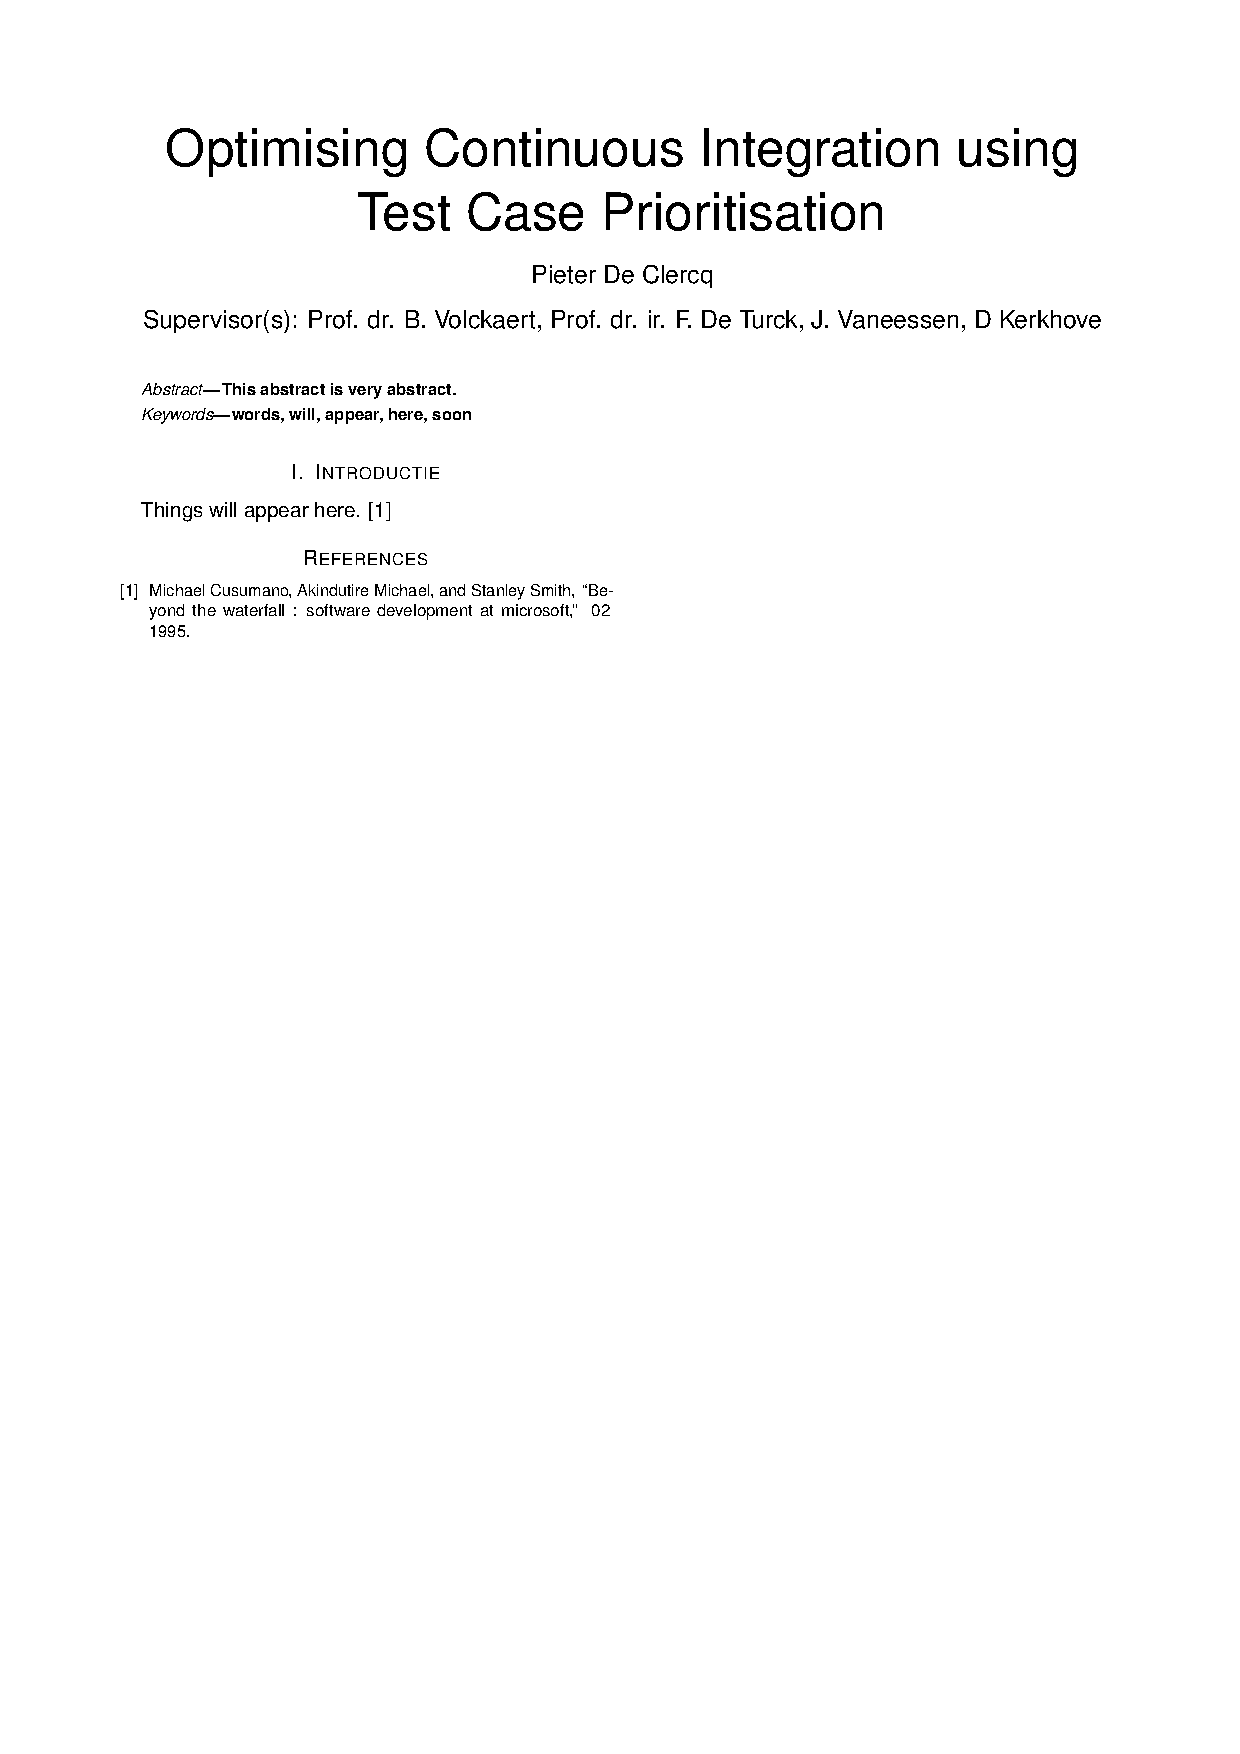
\includepdf[pages=-]{abstract-en/extended-abstract.pdf}
\addcontentsline{toc}{chapter}{Extended abstract (Dutch)}
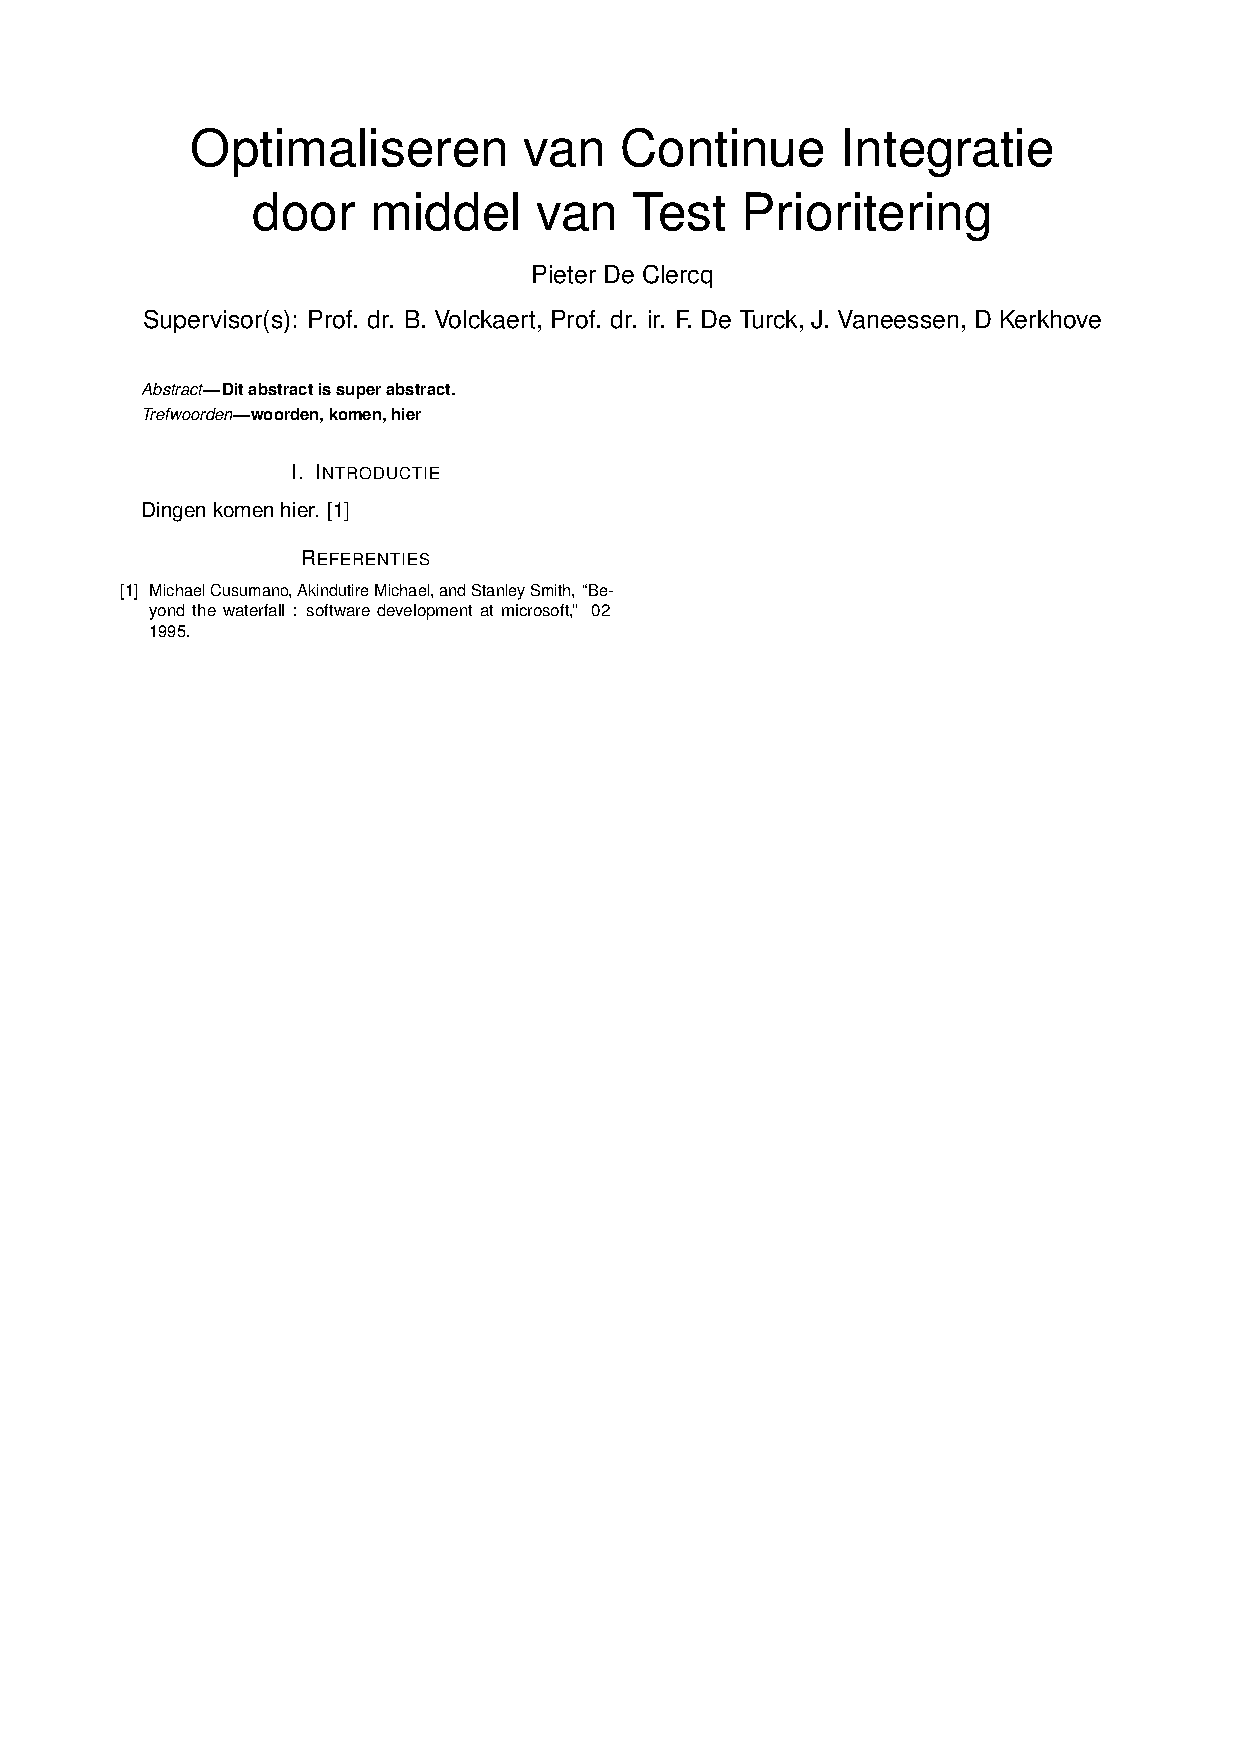
\includepdf[pages=-]{abstract-nl/extended-abstract.pdf}

% Lay summary.
% !TeX root = ../thesis.tex

\chapter*{Lay summary}

\section*{Software}
Every digital device that exists today, from computers, smartphones, cars, to even much simpler devices like alarm clocks and microwaves, consists of two distinct parts. The first, physical part is the hardware, which is the combination of mechanical bits and electrical wiring that enable a device to interact with the real world. The type of interaction can range from either very primitive to extremely complex, such as emitting an LED-light, producing a sound, or launching a rocket. The second part is the software, which is installed on the hardware of the device. Software is developed by software engineers using programming languages and instructs the hardware on what to do, and when.

% entire science on its own is geen ding -> zoek andere uitdrukking
% before they reach the users
\section*{Testing}
Deciding on what is the "best" approach towards the development of software is an entire science on its own with two main conceptions. The traditional approach starts with a thinking phase, followed by a programming phase and finalised by a testing phase. In the first phase, the developers create a detailed design document that describes the required functionality of the final application. Next, the developers write computer code that implements the desired functionality. When this process is completed, the quality assurance team thoroughly tests the application. This testing phase exists in hardware as well. Consider, for example, crash tests conducted by car manufacturers. The purpose of these tests is to detect potential issues and anomalies (bugs) in the application before its end-users do. This phase is critical because bugs can result in financial loss or incur other disastrous effects, such as the explosion of two space rockets in the previous decade, mere seconds after ignition.

\section*{Continuous Integration}
The urge to limit financial losses is even more prominent today, in the wake of the world economic crisis and the more recent COVID-19 induced crisis. While the aforementioned traditional approach works well for small projects, it suffers from severe scalability issues when the size of the application increases at today's pace, since the testing phase consumes valuable time, and time equals money. As a result, software developers have shifted towards an Agile development approach. This approach encourages software developers not to release the entire application at once, but to release an initial version with a reduced functionality set as soon as possible and add extra features iteratively. Additionally, developers must include thorough software tests and execute these every time they make a change, to reduce the probability of introducing bugs. This tedious task can be automated by employing Continuous Integration (CI) software, which automatically executes the test cases after every change to the application code change, as illustrated in \Cref{fig:ci}.

\begin{figure}[h!]
	\centering
	\includegraphics[width=\textwidth]{assets/tikz/ci-simple.tikz}
	\caption{\CI{} (simplified).}
	\label{fig:ci}
\end{figure}

\section*{Scalability}
Nevertheless, Continuous Integration is not a silver bullet. In the initial stage of the project, the number of test cases will be rather small, therefore providing fast feedback to the developers in case of failure. However, as time progresses and the application grows, more test cases will be added that all need to be executed after every change. Eventually, this will consume a significant amount of time as well, thereby nullifying these benefits.

\section*{Solution}
This thesis focuses on resolving this problem by introducing three techniques. The first two techniques are \emph{Test Suite Minimisation} and \emph{Test Case Selection}. These techniques attempt to predict which test cases are likely to fail, and as such, only execute those test cases with a high probability of failing. The third technique is \emph{Test Case Prioritisation (TCP)}. As the name suggests, this technique will execute every test case in a specific sequence. The order of this sequence is determined by the predicted chance that the test case will fail, executing the most likely failing test cases as soon as possible.\\ This thesis concentrates on TCP (\Cref{fig:tcp-lay}) since this technique ensures that every failing test case will eventually be executed. The other two techniques cannot guarantee this because a failing test case might accidentally be omitted. 

% Maak Publish - Release
\begin{figure}[t!]
	\centering
	\includegraphics[width=0.96\textwidth]{assets/tikz/tcp-lay.tikz}
	\caption{\tcp{}.}
	\label{fig:tcp-lay}
\end{figure}

\section*{Prediction}
In order to estimate which test cases might fail, the TCP implementation in this thesis consists of ten prediction algorithms, referred to as predictors. Every predictor uses the same input data but with a different interpretation, which is out-of-scope for this summary. This input data is threefold:
\begin{enumerate}
	\item \textbf{Affected test cases:} The predictors contain a mapping that links every test case to the corresponding tested lines of code in the application. If the developer modifies a line of code, every \emph{affected} test case is considered a potential failure.
	
	\item \textbf{Historical data:} Next, the predictors can examine whether or not a test case has recently failed. Research has indicated that test cases tend to fail consecutively.
	
	\item \textbf{Duration data:} Finally, the predictors can use the average duration of a test case as a tie-breaker. If two test cases are equally likely to fail, the test case with the lowest duration should be preferred in order to speed up the execution.
\end{enumerate}

\section*{Results}
The benefits of applying TCP on two existing applications have been analysed. The results are promising: on average, the implemented framework will only execute $\SIrange{3}{5}{\percent}$ of the test cases before a failure is observed. When examining the time it takes to detect a failing test case, the results indicate a reduction of more than $\SIrange{30}{50}{}$ times compared to the original, unprioritised execution.
\clearpage

\pagestyle{fancy}

\blankpage{}

% ToC.
\tableofcontents

% Corpus.
\mainmatter

% !TeX root = thesis.tex

\printglossary
\clearpage
% !TeX root = thesis.tex

\chapter{Introduction}
Given the complexity and rapid pace at which software is being built today, it is inevitable that at some point bugs will emerge. These bugs can either be introduced by a malfunctioning new feature, or by breaking existing functionality (\emph{a regression}). In order to detect bugs in an application before its customers do, an adequate \emph{testing infrastructure} is required.\\

\noindent This testing infrastructure consists of multiple \emph{test cases}, collectively referred to as the \emph{test suite} of the application. The quality of a test suite can be assessed in multiple ways. The first and most used option is to measure which fraction of the source code is tested by at least one test case, a ratio which is expressed as the \emph{coverage} of the application. Another possibility is to apply transformations to the source code and validate whether or not this results in a failed test case, a process indicated as \emph{mutation testing}.\\

\noindent Ideally, this testing process should be automated and performed after every change to the source code. This is generally a very time-consuming occupation, and as such has led to the creation of various automation frameworks and tools, collected under the name of \emph{Continuous Integration} \texttt{[CI]}. Common examples of CI practices are automatically running the test suite and estimating the code coverage after every pushed change to the \emph{Version Control System} \texttt{[VCS]}.\\

\noindent However, applying these practices and maintaining a qualitative test comes at a cost. After every addition or modification to the source code, at least one new test case must be introduced to validate its correctness. As a result of the speed at which the source code tends to grow, the test suite suffers from severe scalability issues. While it is desired and ideally required to execute every single test case in the test suite, there are examples known to literature where this is not possible since this incurs an increasing delay in the development process, which in turn results in economic loss.\\

\noindent Three approaches can be taken towards resolving this issue by reducing the time occupied by waiting for the test results: \tsm{} \texttt{[TSM]}, \tcs{} \texttt{[TCS]} and \tcp{} \texttt{[TCP]}. The main subject of this thesis will be to implement a framework for TCP. To accomplish this, the next chapter will introduce important concepts which are used in modern software engineering. \autoref{chap:related-work} will elaborate on the aforementioned approaches and present accompanying algorithms. The implementation details of the new framework will be discussed in \autoref{chap:velocity}. Afterwards, \autoref{chap:evaluation} will evaluate the performance of this framework and provide insights to the characteristics of a typical test suite. More specifically, this chapter will research the probability of (repeated) test failure and the average duration of a test run. Finally, \autoref{chap:conclusion} will present additional ideas and improvements to the framework.
\clearpage
% !TeX root = thesis.tex

\chapter{Software Engineering}
\label{chap:software-engineering}
The Institute of Electrical and Electronics Engineers \texttt{[IEEE]} defines the practice of Software Engineering as: "Application of a systematic, disciplined, quantifiable approach to the development, operation and maintenance of software; that is, the application of engineering to software" \cite[p.~421]{8016712}. The word ``systematic'' in this definition, emphasises the need for a structured process, depicting guidelines and models that describe how software should be developed the most efficient way possible. Such a process does exist and it is often referred to as the Software Development Life Cycle (SDLC) \cite[p.~420]{8016712}. In the absence of a model, i.e. when the developer does what they deem correct without following any rules, the term \emph{Cowboy coding} is used \cite[p.~34]{landry2011iterative}.

% !TeX root = ../thesis.tex

\section{Software Development Life Cycle}\label{sec:se-sdlc}
An implementation of the SDLC consists of two parts. The first part is a list of phases, and the second part is a function that describes the transitions between these phases. Depending on the nature of the software, existing phases can either be omitted or additional phases can be added. The five phases below were compiled from multiple sources \cite{2010govardhan, 7106435} and describe a generic approach to which most software projects adhere.
\begin{enumerate}
	\bolditem{Requirements phase} In the first phase of the development process, the developers acquaint themselves with the project and compile a list of the desired functionalities \cite{7106435}. Subsequently, the developers can decide on the financial details, the required hardware specifications as well as which external software libraries will need to be acquired.
	
	\bolditem{Design phase} After the developer has gained sufficient knowledge about the project requirements, they can use this information to construct an architectural design of the application. This design consists of multiple documents, such as user stories and UML-diagrams. A user story describes which actions can be performed by which users, whereas a UML-diagram specifies the technical interaction between the individual components.
	
	\bolditem{Implementation phase} In the third phase, the developers will write code according to the specifications defined in the architectural designs.
	
	\bolditem{Testing phase} The fourth phase is the most critical. This phase will require the developers and quality assurance managers to test the implementation of the application thoroughly. The goal of this phase is to identify potential bugs before the application is made available to other users.
	
	\bolditem{Operational phase} The final phase marks the completion of the project, after which the developers can integrate it into the existing business environment of their customer.
\end{enumerate}

\noindent After we have identified the phases, we must define the transition from one phase into another phase using a model. Multiple models exist in the literature \cite{2010govardhan}, with each model having its advantages and disadvantages. This thesis will consider the traditional model, which is still widely used as of today. The base of this model is the Waterfall model by Benington  \cite{united1956symposium}. Similar to a real waterfall, this model executes every phase in cascading order. However, this imposes several restrictions. The most prevalent issue is the inability to revise a design decision when performing the actual implementation. To mitigate this problem, Royce has proposed an improved version of the Waterfall model \cite{Royce:1987:MDL:41765.41801}, which does allow a phase to transition back to any preceding phase. \Cref{fig:waterfall-royce} illustrates this updated model.

\begin{figure}[htbp!]
	\includegraphics[width=\textwidth]{assets/tikz/waterfall-model.tikz}
	\caption{Improved Waterfall model by Royce}
	\label{fig:waterfall-royce}
\end{figure}

\noindent The focus of this thesis will be on the implementation and testing phases, as these are the most time-consuming phases of the entire process. The modification that Royce has applied to the Waterfall model is particularly useful when applied to these two phases in the context of \emph{software regressions} \cite{10.1007/978-3-540-77966-7_18}. We employ the term ``regression'' when a feature that was once working as intended is suddenly malfunctioning. The culprit of this problem can be a change in the code, but this behaviour can also have an external cause, such as a change in the system clock due to daylight saving time. Sometimes, a regression can even be the result of a change to another, seemingly unrelated part of the application code \cite{6588537}.

\subsection{Taxonomy of test cases}

Software regressions and other functional bugs can ultimately incur disastrous effects, such as severe financial loss or permanent damage to the reputation of the software company. The most famous example in history is without any doubt the explosion of the Ariane 5-rocket, which was caused by an integer overflow \cite{581900}. In order to reduce the risk of bugs, we should be able to detect malfunctioning components as soon as possible to warden the application against potential failures before they occur. Consequently, we must consider the testing phase as the most critical phase of the entire development process and therefore include sufficient test cases in the application. The collection of all the test cases in an application is referred to as the \emph{\gls{testsuite}}. We can distinguish many different types of test cases. This thesis will consider three categories in particular.

\subsubsection{Unit tests}
This is the most basic test type. The purpose of a unit test is to verify the behaviour of an individual component \cite{whittaker2000}. As a result, the scope of a unit test is limited to a small and isolated piece of code, e.g. one function. Implementation-wise, a unit test is typically an example of a \gls{whiteboxtest} \cite[p.~12]{6588537}. The term white-box indicates that the creator of the test case can manually inspect the code before constructing the test. As such, they can identify necessary edge values or corner cases. Common examples of these edge values include zero, negative numbers, empty arrays or array boundaries that might cause an overflow. Once the developer has identified the edge cases, they can construct the unit test by repeatedly calling the function under test, each time with a different (edge) argument value, and afterwards verifying its behaviour and result. These verifications are referred to as \emph{assertions}. \Cref{lst:se-unit-test} contains a unit test written in Java using the popular JUnit test framework.\\
	
\lstinputlisting[caption=Java unit test in JUnit., label=lst:se-unit-test, language=Java]{assets/listings/example-unit-test.java}

\clearpage

\subsubsection{Integration tests}
The second category involves a more advanced type of tests. An integration test validates the interaction between two or more individual components \cite{whittaker2000}. Ideally, accompanying unit tests should exist that test these components as well. As opposed to the previous unit tests, a developer will usually implement an integration test as a \gls{blackboxtest} \cite[p.~6]{6588537}. The difference between a black-box and a white-box test is that a black-box test assumes that the implementation details of the code under test are unknown during the construction of the test. Since a black-box test does not require any details about the code, we can, in fact, construct the integration tests before we implement the actual feature itself. A typical example of an integration test is the communication between the front-end and the back-end side of a web application. Another example is illustrated in \Cref{lst:se-integration-test}.\\
	
\lstinputlisting[caption=Java integration test in JUnit., label=lst:se-integration-test, language=Java]{assets/listings/example-integration-test.java}

\clearpage

\subsubsection{Regression tests}
After a developer has detected a regression in the application, they will add a regression test \cite[p.~372]{8016712} to the test suite. This regression test must replicate the exact conditions and sequence of actions that have triggered the failure. The goal of this test is to prevent similar failures to occur in the future if the same conditions would reapply. An example is provided in \Cref{lst:se-regression-test}.\\

\lstinputlisting[caption=Java regression test in JUnit., label=lst:se-regression-test, language=Java]{assets/listings/example-regression-test.java}
% !TeX root = ../thesis.tex

\section{Agile Software Development}
% !TeX root = ../../thesis.tex

\subsection{Agile Manifesto}
Since the late 1990s, developers have tried to reduce the time occupied by the implementation and testing phases. As a result, several software pioneers have proposed new implementations of the SDLC, which were later collectively referred to as the \emph{Agile development methodologies}. This term was coined during a meeting of seventeen prominent software developers, in which they have defined the following four fundamental values of Agile development in the \emph{Agile Manifesto} \cite{beck2001agile}.

\begin{enumerate}
	\item \emph{Individuals and interactions} over processes and tools.
	\item \emph{Working software} over comprehensive documentation.
	\item \emph{Customer collaboration} over contract negotiation.
	\item \emph{Responding to change} over following a plan.
\end{enumerate}

\noindent According to the authors, we should interpret these values as follows: ``While there is value in the items on the right, we value the items on the left more'' \cite{beck2001agile}. When we examine these values more closely, we can observe that they all share a common philosophy, which is that software engineering should be a fast process in which communication and a short feedback loop is critical to avoid missteps. Since 2001, a variety of different programming models have arisen, each incorporating these agile principles in their own way. The most remarkable new practice is \acrfull{tdd}. Recall that an integration test is a black-box test and that as such, we can actually construct the test case in advance and write the implementation afterwards. This concept is also prevalent in TDD. This practice depicts that if we want to extend the functionality of the application, we should first modify the test cases (or add new test cases) and then modify the application code until every test case is passing \cite{10.5555/579193}.
% !TeX root = ../../thesis.tex

\subsection{The need for Agile}
In the wake of the world economic crisis, software companies were forced to devote efforts into researching how their overall expenses could be reduced. This research has concluded that in order to reduce financial risks, the \emph{time-to-market} of an application should be as short as possible. In order to accomplish this, further research was conducted, resulting in an increase of attention for agile methodologies in scientific literature \cite{ionel2009}. As was previously described in \autoref{sssec:agilevalue-workingsoftware}, agile methodologies strive to deliver a minimal version as soon as possible, allowing additional functionality to be added in an incremental fashion. This effectively results in a shorter \emph{time-to-market} and lower costs, since the company can decide to cancel the project much earlier in the process.\\

\noindent In addition to a reduced time-to-market, maintaining an agile workflow has also proven beneficial to the success rate of development. A study performed by The Standish Group revealed that the success rate of agile projects is more than three times higher compared to when traditional methodologies are practised \cite[p.~7]{standish2015chaos}, as illustrated in \autoref{fig:agile-success-rate}. 

\begin{figure}[htbp!]
	\centering
	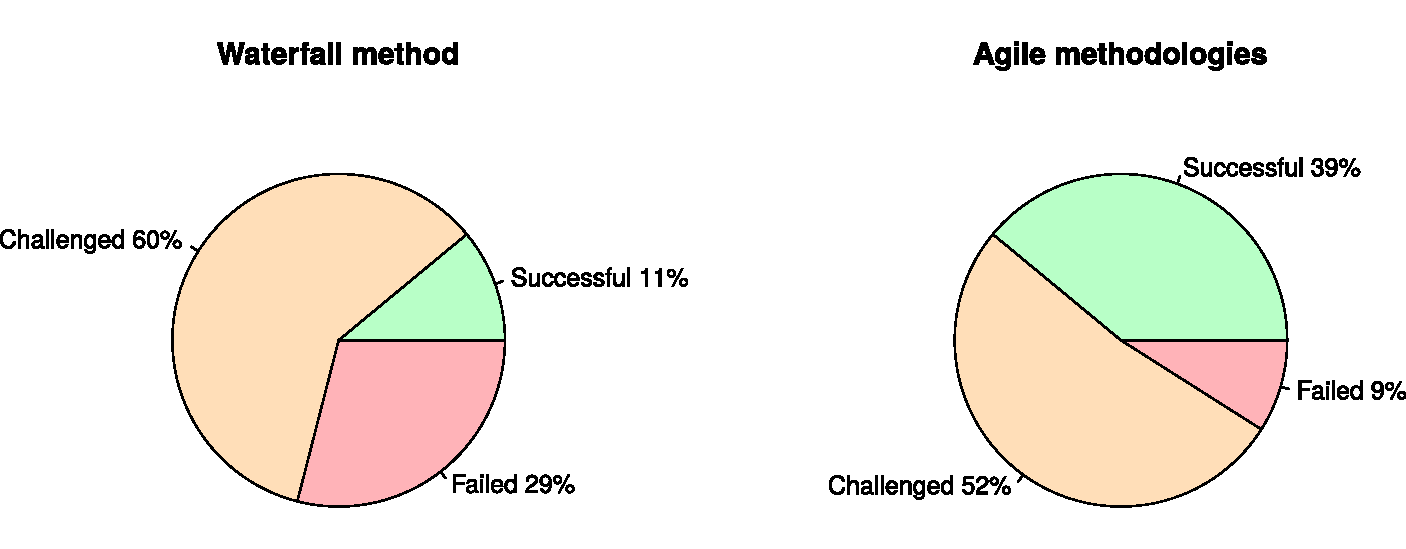
\includegraphics[width=\textwidth]{assets/agile-success-rate.pdf}
	\caption{Success rate of Agile methodologies \cite{standish2015chaos}.}
	\label{fig:agile-success-rate}
\end{figure}



%hier in hoofdstuk 7 staat iets over continuous integration
%https://link.springer.com/chapter/10.1007/978-3-319-05155-0_7

- changes moeten zeer regelmatig worden geintegreerd met elkaar -> feedback loop tussen implement -> integrate -> test -> repeat
- Continuous integration: wat?
- Bestaan aantal bestaande frameworks voor
- Maar; dat testen kan heel lang duren (zoek een bron waarin lange tests besproken worden)
- Bestaan aantal oplossingen voor -> zie volgende hoofdstuk

- feedback loop

- buildup naar waarom tooling nodig is

- waarom

- wat

- voorbeelden: Jenkins, CircleCI, Travis-CI, recent GitHub Actions + screenshots

- Probleem en oplossingen met regression tests


\section{Continuous Integration}
\subsection{Agile Manifesto}
Since the late 1990's, developers have tried to reduce the time occupied by the implementation and testing phases. In order to accomplish this, several new implementations of the SDLC were proposed and evaluated, later collectively referred to as \emph{Agile development methodologies}. The term \emph{Agile development} was coined during a meeting of seventeen prominent software developers, held between February 11-13, 2001, in Snowbird, Utah \cite{jimhighsmith2001}. As a result of this meeting, the developers defined the four key values and twelve principles that define these new methodologies, called the \emph{Manifesto for Agile Software Development}, also known as the \emph{Agile Manifesto}.\\

\noindent The four key values of Agile software development should be interpreted as follows, according to the authors: "While there is value in the items on the right, we value the items on the left more" \cite{beck2001agile}. I will explain these key values and their corresponding principles, as proposed by Kiv \cite[p.~12]{10.1007/978-3-030-03673-7_2}. It should be noted that these values are merely guidelines and that no concrete implementation is provided. A variety of different programming models, based on the agile ideologies, have arisen since 2001, each incorporating these values and principles in their own unique way.

\subsubsection{\emph{Individuals and interactions} over processes and tools}
Instead of meticulously following an outlined development process and utilising the best tools available, the main focus of attention should shift to the people behind the development and how they are interacting with each other. According to Glass, the quality of the programmers and the team is the most influential factor in the successful development of software \cite{glass2001agile}. 

\agileprinciple{5}{Build projects around motivated individuals. Give them the environment and support they need, and trust them to get the job done.}
TODO EXPLAIN

\agileprinciple{6}{The most efficient and effective method of conveying information to and within a development team is face-to-face conversation.}
TODO EXPLAIN

\agileprinciple{8}{Agile processes promote sustainable development. The sponsors, developers, and users should be able to maintain a constant pace indefinitely.}
TODO EXPLAIN

\agileprinciple{11}{The best architectures, requirements, and designs emerge from self-organizing teams.}
TODO EXPLAIN

\agileprinciple{12}{At regular intervals, the team reflects on how to become more effective, then tunes and adjusts its behavior accordingly.}
TODO EXPLAIN

\subsubsection{\emph{Working software} over comprehensive documentation}
The primary goal of software engineering is to deliver a working end product which fulfils the needs of the customer. In order to accomplish this, development should start as soon as possible. Traditional programming models demand a lot of documentation to be written prior to the actual development, which will inevitably lead to inconsistencies between the documentation and the actual application as the project grows and the requirements change \cite{Hazzan2014}. 
	
\agileprinciple{1}{Our highest priority is to satisfy the customer through early and continuous delivery of valuable software.}
TODO EXPLAIN

\agileprinciple{3}{Deliver working software frequently, from a couple of weeks to a couple of months, with a preference to the shorter timescale.}
TODO EXPLAIN

\agileprinciple{7}{Working software is the primary measure of progress.}
TODO EXPLAIN

\agileprinciple{10}{Simplicity--the art of maximizing the amount of work not done--is essential.}
TODO EXPLAIN

\subsubsection{\emph{Customer collaboration} over contract negotiation}
In traditional software engineering, the role of the customer is subordinate to the developer. Agile software engineering maintains a different perception of this role, treating both the customer and developers as equal entities. Daily contact between both parties is of vital importance to avoid misunderstandings and a short feedback loop allows the developers to cope with changes in requirements and to ensure that the customer is satisfied with the delivered product \cite{Hazzan2014}.

\agileprinciple{4}{Business people and developers must work together daily throughout the project.}
TODO EXPLAIN

\subsubsection{\emph{Responding to change} over following a plan}
The first step of the aforementioned waterfall model (\autoref{sec:se-sdlc}) was to ensure both the customer and the developers have a complete and exhaustive view of the entire application. In reality however, this has proven to be rather difficult and sometimes even impossible. As a result of this, a change in requirements was one of the most common causes of software project failure \cite{glass2001agile}. Consequently, the agile software development methodologies do not require a complete specification of the final product to be known a priori and stimulate the developers to successfully cope with changes as the application is being developed \cite{Hazzan2014}. This is accomplished by working in short iterations (sprints), instead of programming the entire application at once, which is the case with the traditional programming models.

\agileprinciple{2}{Welcome changing requirements, even late in development. Agile processes harness change for the customer's competitive advantage.}
TODO EXPLAIN

\agileprinciple{9}{Continuous attention to technical excellence and good design enhances agility.}
TODO EXPLAIN

\subsection{The need for Agile}
Over the past decade, the agile methodologies have received increasing attention amongst software developers, following the world economic crisis of 2009 \cite{ionel2009}. A consequence of this crisis was that software companies were forced to cut on their expenses and find ways to reduce the \emph{time-to-market} of their applications.

- probleem met waterfall model -> een bron hiervoor?

- feedback loop

- buildup naar waarom tooling nodig is

- waarom

- wat

- voorbeelden: Jenkins, CircleCI, Travis-CI, recent GitHub Actions + screenshots

- Probleem en oplossingen met regression tests

  - Test Case Prioritization -> Focus want geen tests weggooien
  
  - Test Suite Minimization
  
  - Test Suite Selection
  
  - Test Suite Reduction


\clearpage
\chapter{Related work}
- In vorig hoofdstuk uitgelegd dat je vaak moet changes integreren -> vaak tests uitvoeren, maar dat kan miserie zijn als tests heel lang duren want dan ben je maar steeds bezig met wachten tot die tests stoppen

(TODO)

- Maar; dat testen kan heel lang duren (zoek een bron waarin lange tests besproken worden)

- Bestaan aantal oplossingen voor:

  - Test Case Prioritization $\Rightarrow$ Dit doen we, want geen tests weggooien

- Test Suite Minimization

- Test Suite Selection

- Test Suite Reduction

- OpenClover (enkel Java) heeft hier misschien support voor

- Machine Learning approaches

- Heuristieken
\clearpage
% !TeX root = thesis.tex

\chapter{Proposed framework: \velocity{} [TODO REVISE]}
\label{ch:velocity}
The implementation part of this thesis consists of a framework and a set of tools, tailored at optimising the test suite as well as providing accompanying metrics and insights. The framework was named \emph{\velocity{}} to reflect its purpose of enhancing the speed at which \CI{} is practised. This paper will now proceed by describing the design goals of the framework. Afterwards, a high-level schematic overview of the implemented architecture will be provided, followed by a more in-depth explanation of every pipeline step. In the final section of this chapter, the \emph{Alpha} algorithm will be presented.

% !TeX root = ../thesis.tex

\section{Design goals}
\velocity{} has been implemented with four design goals in mind:
\begin{enumerate}
	\item \textbf{Extensibility:} It should be possible and straightforward to support additional CI systems, programming languages and test frameworks. Similarly, a clear interface must be provided to integrate new prioritisation algorithms.
	
	\item \textbf{Minimally invasive:} Integrating \velocity{} into an existing test suite should not require drastic changes to any of the test cases.
	
	\item \textbf{Language agnosticism:} This design goal is related to the extensibility of the framework. The implemented tools should not need to be aware of the programming language of the source code, nor the used test framework.
	
	\item \textbf{Self-improvement:} The prioritisation framework must support multiple algorithms. However, the performance of an algorithm might be dependent on the nature of the source code. An algorithm may offer a very high accuracy on one project but fall short on another. The framework should decide by itself which algorithm it should prefer, by measuring the performance of a prediction and subsequently infer which algorithm to use for future predictions.
\end{enumerate}
% !TeX root = ../thesis.tex

\section{Architecture}

\begin{figure}[htbp!]
	\centering
	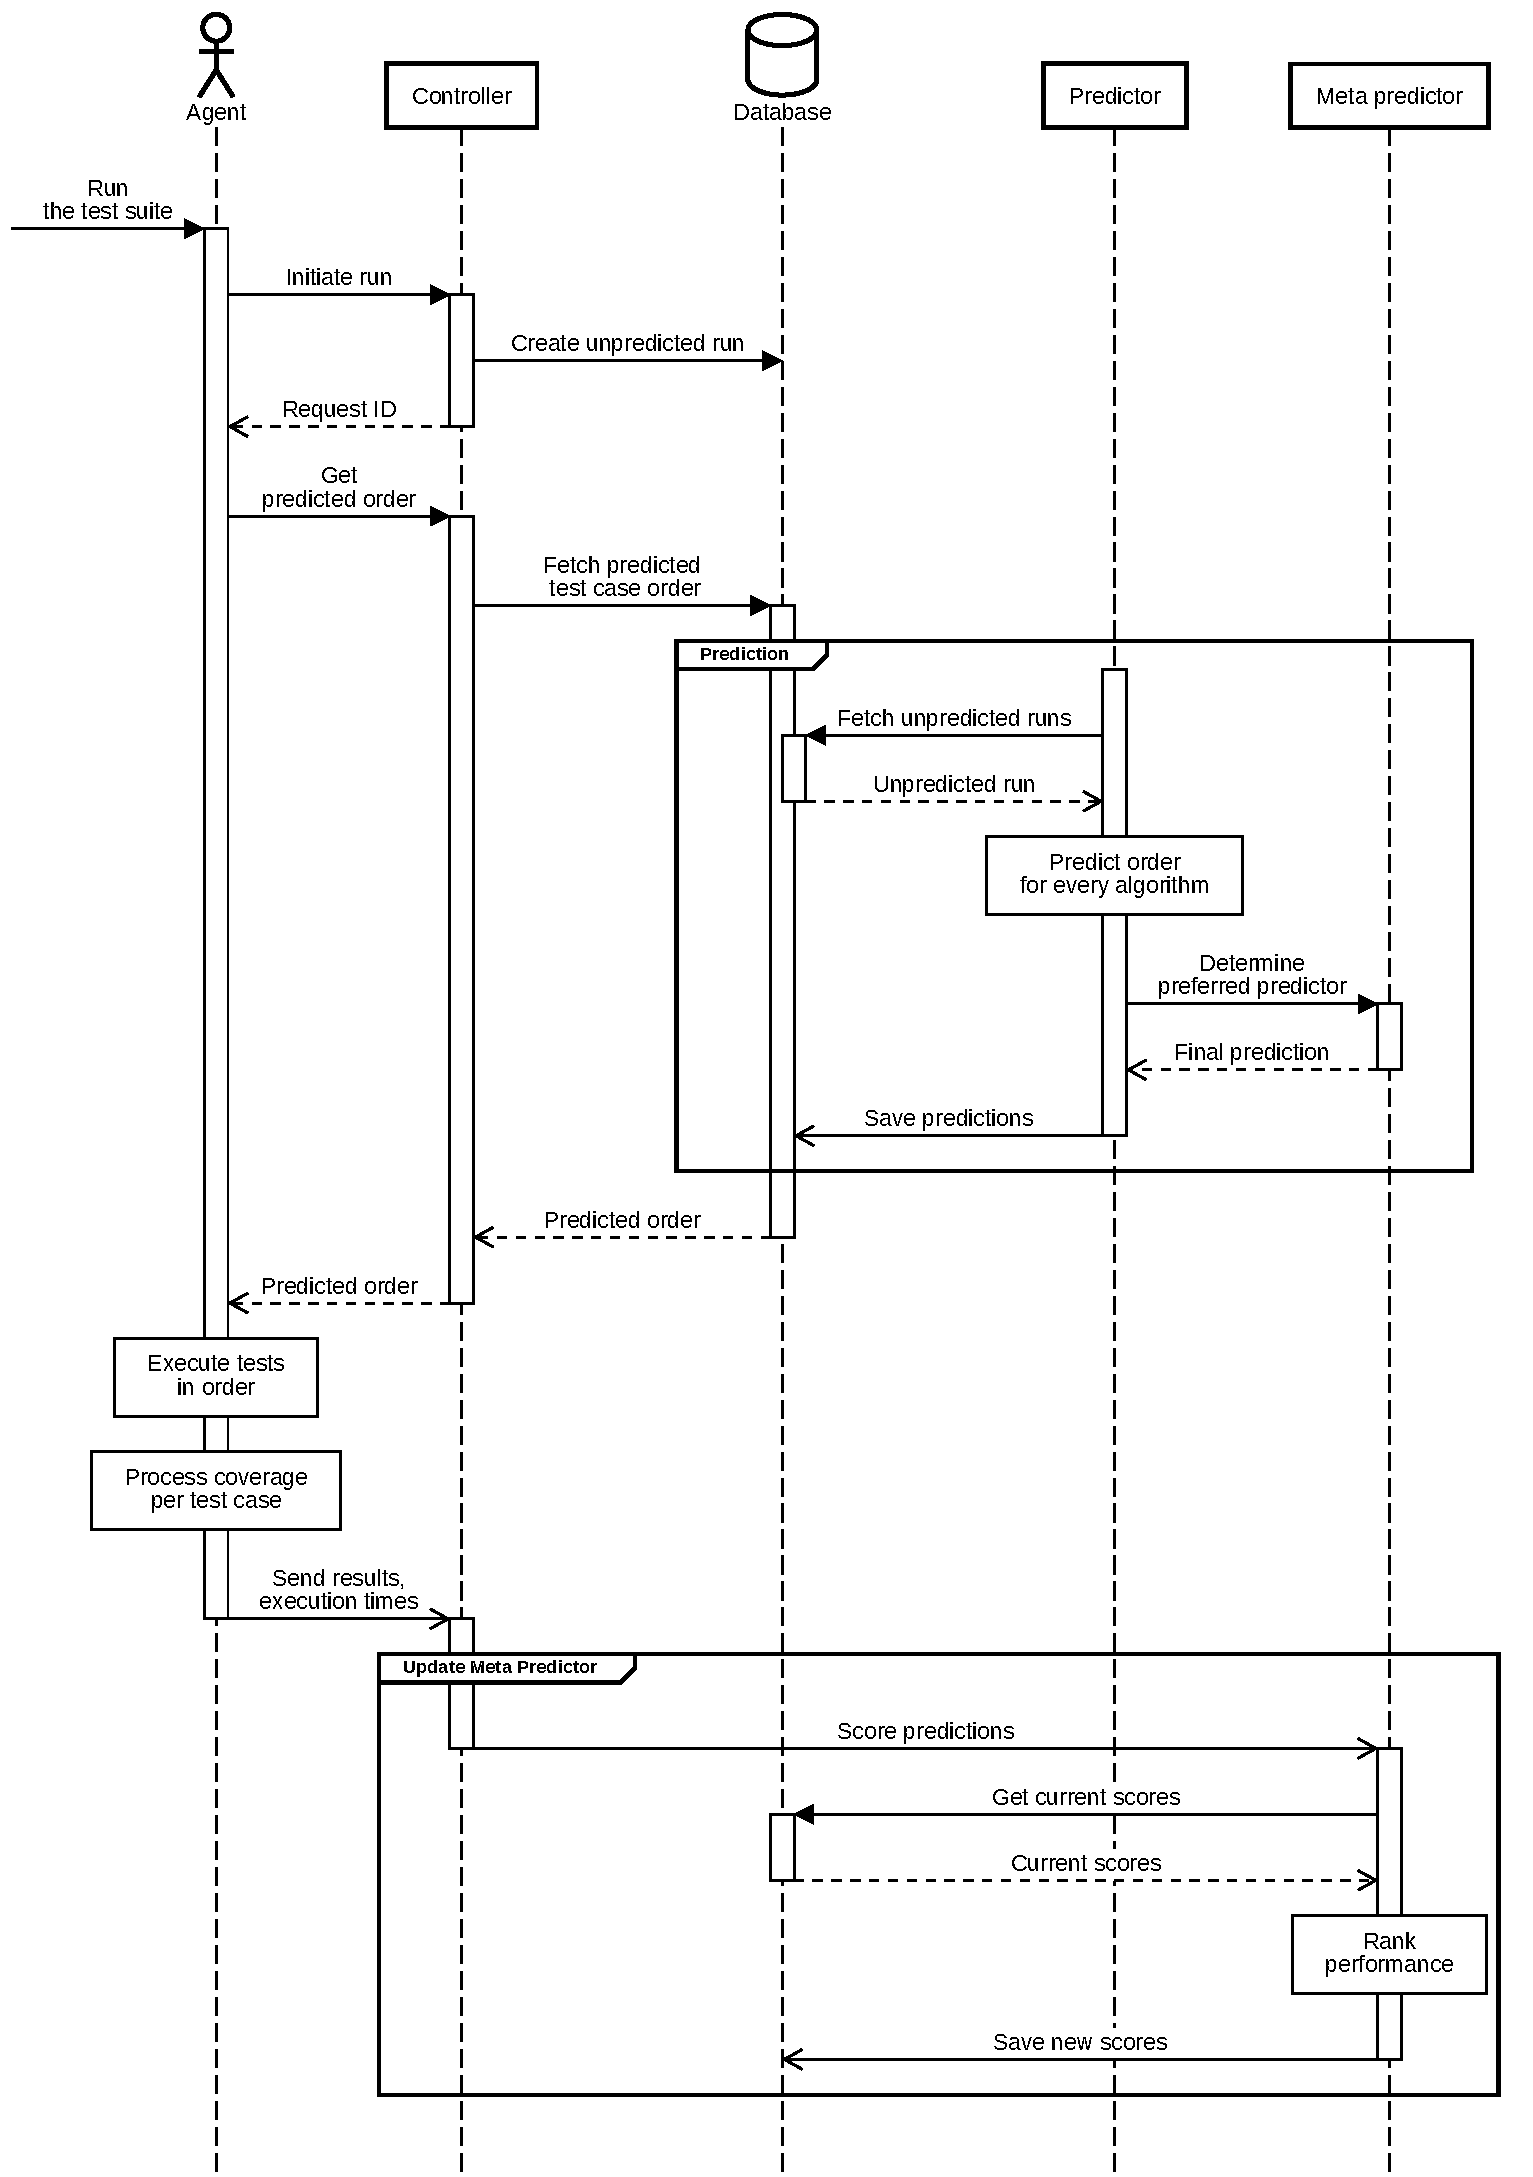
\includegraphics[height=\textheight]{assets/diagrams/sequence-diagram.pdf}
	\caption{Sequence diagram of \velocity{}}
	\label{fig:velocity-sequence-diagram}
\end{figure}

\subsection{Agent}
\label{ssec:velocity-frontend}
The first component that we will consider is the agent. The agent interacts directly with the source code and the test suite and is, therefore, the only component that is specific to the programming language and the test framework. Every programming language and test framework requires a different implementation of the agent, although these implementations are strongly related. This thesis provides a Java agent, which is available as a plugin for the Gradle and JUnit test framework, a combination which has previously been described in \cref{ssec:relatedwork-gradle-junit}. When the test suite is started, the plugin will contact the controller (\cref{ssec:velocity-controller}) to obtain the prioritised test case order and subsequently execute the test cases in that order. Afterwards, the plugin will send a feedback report to the controller, where it is analysed.

\subsection{Controller}\label{ssec:velocity-controller}
The second component is the core of the framework, acting as an intermediary between the agent on one side and the predictor (\cref{ssec:velocity-predictor}) on the other side. In order to satisfy the second design goal and as such allow language agnosticism, the controller exposes a \Gls{rest}-interface, to which the agent can communicate using the \texttt{HTTP} protocol. On the other side, the controller does not communicate directly with the predictor but stores prediction requests in a shared database instead. The predictor will periodically poll this database and update the request with the predicted order. Besides providing routing functionality between the agent and the predictor, the controller is additionally responsible for updating the meta predictor (\cref{ssec:pipeline-postanalysis}) by evaluating the accuracy of earlier predictions.

\subsection{Predictor and Metrics}\label{ssec:velocity-predictor}
The final component is the predictor. The predictor is responsible for applying the prioritisation algorithms to predict the optimal execution order of the test cases. This order is calculated by first executing ten prioritisation algorithms and subsequently consulting the meta predictor to determine the preferred sequence. The predictor has been implemented in Python, because of its accessibility and compatibility with various existing libraries such as NumPy\footnote{\url{https://numpy.org/}} and TensorFlow\footnote{\url{https://www.tensorflow.org/}}, to allow advanced prioritisation algorithms. 
% !TeX root = ../thesis.tex

\section{Pipeline}
This section will elaborate on the individual steps of the pipeline. The steps will be discussed by manually executing the pipeline that has hypothetically been implemented on a Java project. For the sake of simplicity, this explanation will assume a steady-state situation, ensuring the existence of at least one completed run of this project in the database at the controller side.

\subsection{Initialisation}\label{ssec:pipeline-initialisation}
As was explained before, the provided Java implementation of the agent was designed to be used in conjunction with Gradle. In order to integrate \velocity{} into a Gradle project, the build script (\texttt{build.gradle}) should be modified in two places. The first change is to include and apply the plugin in the header of the file. Afterwards, the plugin requires three properties to be configured:
\begin{itemize}
	\item \texttt{base} the path to the Java source files, relative to the location of the build script. This will typically resemble \texttt{src/main/java}.
	
	\item \texttt{repository} the url to the git repository at which the project is hosted. This is required in subsequent steps of the pipeline, to detect which code lines have been changed in the commit currently being analysed.
	
	\item \texttt{server} the url at which the controller can be reached.
\end{itemize}

\noindent \autoref{lst:pipeline-buildgradle} contains a minimal integration of the agent in a Gradle build script, applied to a library for generating random numbers\footnote{\url{https://github.com/thepieterdc/random-java}}. The controller is hosted at the same host as the agent and is accessible at port \texttt{8080}.

\lstinputlisting[caption=Minimal Gradle buildscript, label=lst:pipeline-buildgradle, language=Groovy]{assets/listings/build.gradle}

\noindent After the project has been configured, the test suite must be executed. For the Gradle agent, this involves executing the built-in \texttt{test} task. This task requires an additional argument to be passed, which is the commit hash of the changeset to prioritise. In every discussed \CI{} system, this commit hash is available as an environment variable.\\

\noindent The first step is for the agent to initiate a new test run in the controller. This is accomplished by sending a \texttt{POST}-request to the \texttt{/runs} endpoint of the controller, which will reply with an identifier. On the controller side, this request will result in a new prioritisation request being enqueued in the database that will asynchronously be processed by the predictor daemon in the next step.

\subsection{Prediction}
The prediction of the test execution order is performed by the predictor daemon. This daemon continuously polls the database to fetch new test runs that need to be predicted. When a new test run is detected, the predictor executes every available prediction algorithm in order to obtain multiple prioritised test sequences. The following algorithms are available:

\paragraph*{AllInOrder} The first algorithm will simply prioritise every test case alphabetically and will be used for for benchmarking purposes in \autoref{chap:evaluation}.

\paragraph*{AllRandom} The second algorithm has also been implemented for benchmarking purposes. This algorithm will ``prioritise'' every test case arbitrarily.

\paragraph*{AffectedRandom} This algorithm will only consider the test cases that cover source code lines which have been modified in the current commit. These test cases will be ordered randomly, followed by the other test cases in the test suite in no particular order.

\paragraph*{GreedyCoverAll} The first of three implementations of the Greedy algorithm (\autoref{ssec:alg-greedy}) will execute the algorithm to prioritise the entire test suite.

\paragraph*{GreedyCoverAffected} As opposed to the previous greedy algorithm, the second Greedy algorithm will only consider test cases covering changed source code lines to be prioritised. After these test cases, the remaining test cases in the test suite will be ordered randomly.

\paragraph*{GreedyTimeAll} Instead of greedily attempting to cover as many lines of the source code using as few tests as possible, this implementation will attempt to execute as many tests as possible, as soon as possible. In other words, this algorithm will prioritise test cases based on their average execution time.

\paragraph*{HGSAll} This algorithm is an implementation of the algorithm presented by Harrold, Gupta and Soffa (\autoref{ssec:alg-hgs}). It is executed for every test case in the test suite.

\paragraph*{HGSAffected} Similar to the \emph{GreedyAffected} algorithm, this algorithm is identical to the previous \emph{HGSAll} algorithm besides that it will only prioritise test cases covering changed source code lines.

\paragraph*{ROCKET} The penultimate algorithm is a straightforward implementation of the pseudocode provided in \autoref{ssec:alg-rocket}.

\paragraph*{Alpha} The final algorithm has been inspired by the other implemented algorithms. \autoref{sec:velocity-alpha} will further elaborate on the details.\\

\noindent Subsequently, the final prioritisation order is determined by applying the meta predictor. Essentially, the meta predictor can be seen as a table which assigns a score to every algorithm, indicating its performance on this codebase. \autoref{ssec:pipeline-postanalysis} will explain later how this score is updated. The predicted order by the algorithm with the highest score is eventually elected by the meta predictor as the final prioritisation order, and saved to the database.

\subsection{Test case execution}
Regarding the agent, the identifier obtained in \autoref{ssec:pipeline-initialisation} is used to poll the controller by sending a \texttt{GET} request to \texttt{/runs/id}, which will reply with the test execution order if this has already been determined. One of the discussed features of Gradle in \autoref{ssec:relatedwork-gradle-junit} was the possibility to execute test cases in a chosen order by adding annotations. However, this feature cannot be used to implement the Java agent, since it only supports ordering test cases within the same test class. In order to facilitate complete control over the order of execution, a custom \texttt{TestProcessor} and \texttt{TestListener} have been implemented.\\

\noindent The \texttt{TestProcessor} is responsible for processing every test class in the classpath and forward it along with configurable options to a delegate processor. The final processor in this chain will eventually perform the actual execution of the test class. Since the delegate processors that are built into Gradle will by default execute every method in the test class, the custom processor needs to work differently. The implemented agent will first store every received test class into a list and load the class to obtain all test cases in the class using reflection. After all classes have been processed, the processor will iterate over the prioritised order. For every test case $t$ in the order, the delegate processor is called with a tuple of the corresponding test class and an options array which excludes every test case except $t$. This will effectively forward the same test class multiple times to the delegate processor, but each time with an option that restricts test execution to the prioritised test case, resulting in the desired behaviour.\\

\noindent Subsequently, the \texttt{TestListener} is a method that is called before and after every invocation of a test case. This listener allows the agent to calculate the duration of every test case, as well as collect the intermediary coverage and save this on a per-test case basis.

\subsection{Post-processing and analysis}\label{ssec:pipeline-postanalysis}
The final step of the pipeline is to provide feedback to the controller, to evaluate the accuracy of the predictions and thereby implementing the fourth design goal of self-improvement. After executing all test cases, the agent sends the test case results, the execution time and the coverage per test case to the controller by issuing a \texttt{POST} request to \texttt{/runs/id/test-results} and \texttt{/runs/id/coverage}.\\

\noindent Upon receiving this data, the controller will update the meta predictor using the following procedure. The meta predictor is only updated if at least one of the test cases has failed, since the objective of \tcp{} is to detect failures as fast as possible, thus every prioritised order is equally good if there are no failures at all. If however a test case did fail, the predicted orders are inspected to calculate the duration until the first failed test case for every order. Subsequently, the average of all these durations is calculated. Finally, the score of every algorithm that predicted a below average duration until the first failure is increased, otherwise it is decreased. This will eventually lead to the most accurate algorithms being preferred in subsequent test runs.
% !TeX root = ../thesis.tex

\section{Alpha algorithm}
Besides the algorithms which have been presented in \autoref{sec:relatedwork-algorithms}, an additional algorithm has been implemented: the \emph{Alpha} algorithm. This was constructed by examining the philosophy behind every discussed algorithm and subsequently combining the best ideas into a novel prioritisation algorithm. The specification below will assume the same naming convention as described in \autoref{def:alg-naming}. The pseudocode is provided in Algorithm \ref{alg:alpha}\\

\noindent The algorithm consumes the following inputs:
\begin{itemize}
	\item the set of all $n$ test cases: $TS = \{T_1, \dots, T_n\}$
	
	\item the set of $m$ \emph{affected} test cases: $AS = \{T_1, \dots, T_m\} \subseteq TS$. A test case $t$ is considered ``affected'' if any source code line which is covered by $t$ has been modified or removed in the commit that is being predicted.
	
	\item $C$: the set of all lines in the application source code, for which a test case $t \in TS$ exists that covers this line and that has not yet been prioritised. Initially, this set contains every covered source code line.
	
	\item the failure status of every test case, for every past execution out of $k$ executions of that test case: $F = \{F_1, \dots, F_n\}$, where $F_i = \{f_1, \dots, f_k\}$. $F_{tj} = 1$ implies that test case $t$ has failed in execution $current - j$.
	
	\item the execution time of test case $t \in TS$ for run $r \in [1 \dots k]$, in milliseconds: $D_{tr}$.
	
	\item for every test case $t \in TS$, the set $TL_t$ is composed of all source code lines that are covered by test case $t$.
\end{itemize}

\noindent The first step of the algorithm is to determine the execution time $E_t$ of every test case $t$. This execution time is calculated as the average of the durations of every successful (i.e.) execution of $t$, since a test case will be prematurely aborted upon the first failed assertion, which introduces bias in the duration timings. In case $t$ has never been executed successfully, the average is computed over every execution of $t$.

\[
	E_t = \left.
	\begin{cases}
		\overline{\{D_{ti} \vert i \in [1 \dots k], F_{ti} = 0\}} & \exists j \in [1 \dots k], F_{tj} = 0 \\
		\overline{\{D_{ti} \vert i \in [1 \dots k]\}} & \text{otherwise} \\
	\end{cases}
	\right.
\]

\noindent Next, the algorithm executes every affected test case that has also failed at least once in its three previous executions. This reflects the behaviour of a developer attempting to resolve the bug that caused the test case to fail. Specifically executing \emph{affected} failing test cases first is required in case multiple test cases are failing and the developer is resolving these one by one, an idea which was extracted from the ROCKET algorithm (\autoref{ssec:alg-rocket}). In case there are multiple affected failing test cases, the test cases are prioritised by increasing execution time. After every selected test case, $C$ is updated by subtracting the code lines that have been covered by at least one of these test cases.\\

\noindent Afterwards, the same operation is repeated for every failed but unaffected test case, likewise ordered by increasing execution time. Where the previous step helps developers to get fast feedback about whether or not the specific failing test case they were working on has been resolved, this step ensures that other failing test cases are not forgotten and are executed early in the run as well. Similar to the previous step, $C$ is again updated after every prioritised test case.\\

\noindent Research (TODO reference) has indicated that on average, only a small fraction (TODO PERCENTAGE \%) of all test runs will contain failed tests, resulting in the previous two steps not being executed at all. Therefore, the most time should be dedicated to executing test cases that cover affected code lines. More specifically, the next step of the algorithm executes every affected test case, sorted by decreasing cardinality of the intersection between $C$ and the lines which are covered by the test case. Conforming to the prior two steps, $C$ is also updated to reflect the selected test case. As a consequence of these updates, the cardinalities of these intersections change after every update, which will ultimately lead to affected tests not strictly requiring to be executed. This idea has been adopted from the Greedy algorithm \autoref{ssec:alg-greedy}.\\

\noindent In the penultimate step, the previous operation is repeated in an identical fashion for the remaining test cases, similarly ordered by the cardinality of the intersection with the remaining uncovered lines in $C$.\\

\noindent Finally, the algorithm selects every test case which had not yet been prioritised. Notice that these test cases do not contribute to the test coverage, as every test case that would incur additional coverage would have been prioritised already in the previous step. Subsequently, these test cases are actually redundant and are therefore candidates for removal by \tsm{}. However, since this is a prioritisation algorithm, these tests will still be executed and prioritised by increasing execution time.

\begin{algorithm}[h!]
\caption{Alpha algorithm for \tcp{}}
\label{alg:alpha}
\begin{algorithmic}[1]
	\State {\bfseries Input:} Set $TS = \{T_1, \dots, T_n\}$ of all test cases,
	
	Set $AS = \{T_1, \dots T_m\} \subseteq TS$ of affected test cases,
	
	Set $C$ of all source code lines that are covered by any $t \in TS$,
	
	Execution times $D_{tr}$ of every test case $t$, over all $k$ runs $r$ of that test case,
	
	Failure status $FS$ for each test case over the previous $m$ successive iterations,
	
	Sets $TL = \{TL_1, \dots, TL_n\}$ of all source code lines that are covered by test case $t \in TS$.
	
	\State {\bfseries Output:} Ordered list $P$ of $n$ test cases and their priorities.
	\State $P \gets array[1 \dots n]$ \Comment{initially $0$}
	\State $i \gets n$
	\State $FTS \gets \{t \vert t \in TS \wedge (F[t][1] = 1 \vee F[t][2] = 1 \vee F[t][3] = 1)\}$
	\State $AFTS \gets AS \cap FTS$
	
	\ForAll{$t \in AFTS$} \Comment{sorted by execution time in $E$ (ascending)}
		\State $C \gets C \setminus TL[t]$
		\State $P[t] \gets i$
		\State $i \gets i - 1$
	\EndFor
	
	\State $FTS \gets FTS \setminus AFTS$
	\ForAll{$t \in FTS$} \Comment{sorted by execution time in $E$ (ascending)}
		\State $C \gets C \setminus TL[t]$
		\State $P[t] \gets i$
		\State $i \gets i - 1$
	\EndFor
	
	\State $AS \gets AS \setminus FTS$
	\While{$AS \neq \emptyset$}
		\State $t\_max \gets AS[1]$ \Comment{any element from $AS$}
		\State $tl\_max \gets \emptyset$
		
		\ForAll{$t \in AS$}
			\State $tl\_current \gets C \cap TL_{t}$
			\If{$|tl\_current| > |tl\_max|$}
				\State $t\_max \gets t$
				\State $tl\_max \gets tl\_current$
			\EndIf
		\EndFor
		
		\State $C \gets C \setminus tl\_max$
		\State $P[t] \gets i$
		\State $i \gets i - 1$
	\EndWhile
	
	\State $TS \gets TS \setminus (AS \cup FTS)$
	\While{$TS \neq \emptyset$}
		\State $t\_max \gets TS[1]$ \Comment{any element from $TS$}
		\State $tl\_max \gets \emptyset$
		
		\ForAll{$t \in TS$}
			\State $tl\_current \gets C \cap TL_{t}$
			\If{$|tl\_current| > |tl\_max|$}
				\State $t\_max \gets t$
				\State $tl\_max \gets tl\_current$
			\EndIf
		\EndFor
		
		\State $C \gets C \setminus tl\_max$
		\State $P[t] \gets i$
		\State $i \gets i - 1$
	\EndWhile
	\Return $P$
	
\end{algorithmic}
\end{algorithm}

\clearpage
% !TeX root = thesis.tex

\chapter{Evaluation}
\label{ch:evaluation}
This chapter will evaluate the performance of the framework presented in the previous chapter. The first section introduces the two test subjects that will be used in subsequent experiments. The next section will restate the research questions formally and extend these. Afterwards, we will elaborate on the procedure of the data collection. The final section will provide answers to the research questions as well as present the results of applying \tcp{} to the test subjects.

% !TeX root = ../thesis.tex

\section{Test subjects}

\subsection{Dodona}
Dodona\footnote{\url{https://dodona.ugent.be/}} is an open-source online learning environment created by Ghent University, which allows students from secondary schools and universities in Belgium and South-Korea to submit solutions to programming exercises and receive instant, automated feedback. The application is built using the Ruby-on-Rails web framework. To automate the testing process of the application, Dodona employs \githubactions{} (\cref{sssec:github-actions}) which executes the more than $\SI{450}{}$ test cases in the test suite and performs static code analysis. The application is tested using the default \texttt{MiniTest} testing framework and \texttt{SimpleCov}\footnote{\url{https://github.com/colszowka/simplecov}} is used to record the coverage of the test suite, which is currently approximately $\SI{89}{\percent}$.

\subsection{Stratego}
The second test subject is an application which was created for the Software Engineering Lab 2 course at Ghent University in 2018. The application was created for a Belgian gas transmission system operator and consists of two main components: a web frontend and a backend. This thesis will test the backend in particular since it is written in Java using the Spring framework. Furthermore, the application uses Gradle and JUnit to execute the $\SIrange{300}{400}{}$ test cases in the test suite, allowing the Java agent (\cref{ssec:velocity-frontend}) to be applied directly.
% !TeX root = ../thesis.tex

\section{Research questions}
We will answer the following research questions in the subsequent sections:

\paragraph*{RQ1: What is the probability that a test run will contain at least one failed test case?}
The first research question will provide useful insights into whether a typical test run tends to fail or not. The expectancy is that the probability of failure will be rather low, indicating that it is not strictly necessary to execute every test case and therefore making a case for \tsm{}.

\paragraph*{RQ2: What is the average duration of a test run?}
Measuring how long it takes to execute a typical test run is required to estimate the benefit of applying any form of test suite optimisation. We will only consider successful test runs, to reduce bias introduced by prematurely aborting the execution.

\paragraph*{RQ3: Suppose that a test run has failed, what is the probability that the next run will fail as well?}
The ROCKET algorithm (\cref{ssec:alg-rocket}) relies on the assumption that if a test case has failed in a given test run, it is likely to fail in the subsequent run as well. This research question will investigate the likelihood of this hypothesis.

\paragraph*{RQ4: How can \tcp{} be applied to Dodona and what is the resulting performance benefit?}
This research question will investigate the possibility to apply the \velocity{} framework to the Dodona project and analyse how quickly the available predictors can discover a failing test case.

\paragraph*{RQ5: Can the Java agent be applied to Stratego?}
Since the testing framework used by Stratego should be supported natively by the Java agent, this research question will verify its compatibility. Furthermore, we will analyse the prediction performance, albeit with a small number of relevant test runs.
% !TeX root = ../thesis.tex

\section{Data collection}\label{sec:eval-data}

% !TeX root = ../../thesis.tex

\subsection{\travisci{} build data}
In order to answer the first three research questions, build data for several projects hosted on \travisci{} (\autoref{sssec:travisci}) was used. This data was obtained from two sources.\\

\noindent The first source is a database of $\SI{35793144}{}$ jobs, provided by Durieux et al \cite{travisanalysis}. Due to the magnitude of this dataset ($\SI{61.11}{\gibi\byte}$), a big data framework is required to parse the log files. In order to collect the required data to provide an answer to the first and third research question, two simple \texttt{MapReduce} pipelines have been executed using the Apache Spark\footnote{\url{https://spark.apache.org/}} framework..\\

\begin{figure}[htbp!]
	\centering
	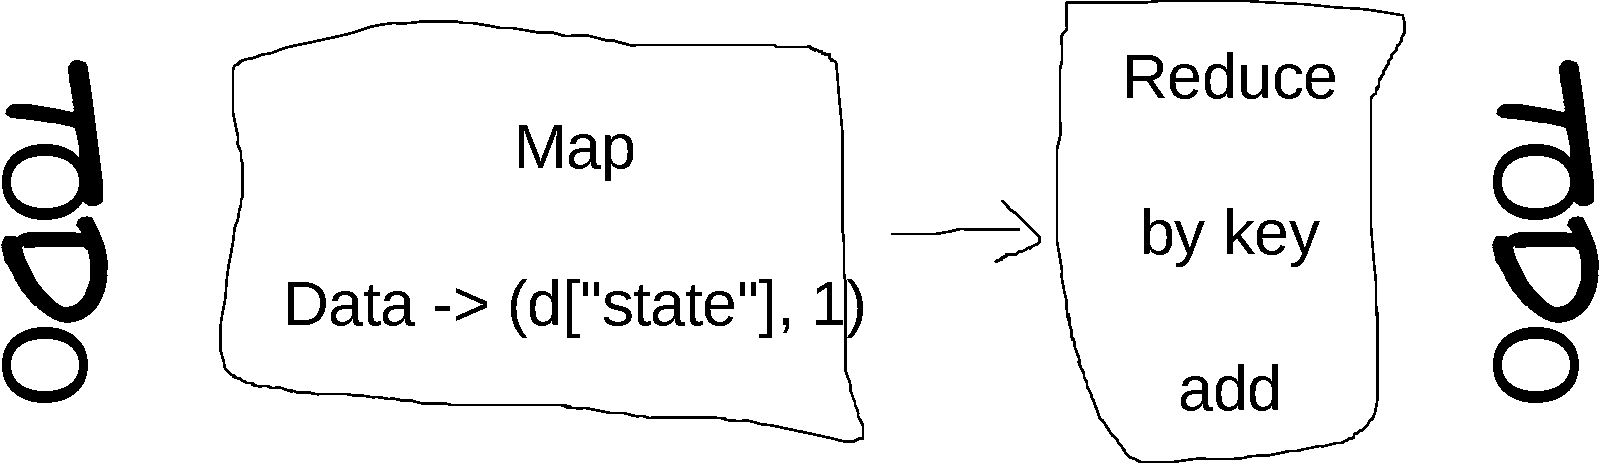
\includegraphics[width=0.8\textwidth]{assets/images/eval-rq1-mapreduce.pdf}
	\caption{MapReduce pipeline to find the failed runs}
	\label{fig:eval-mapreduce-1}
\end{figure}

\begin{figure}[htbp!]
	\centering
	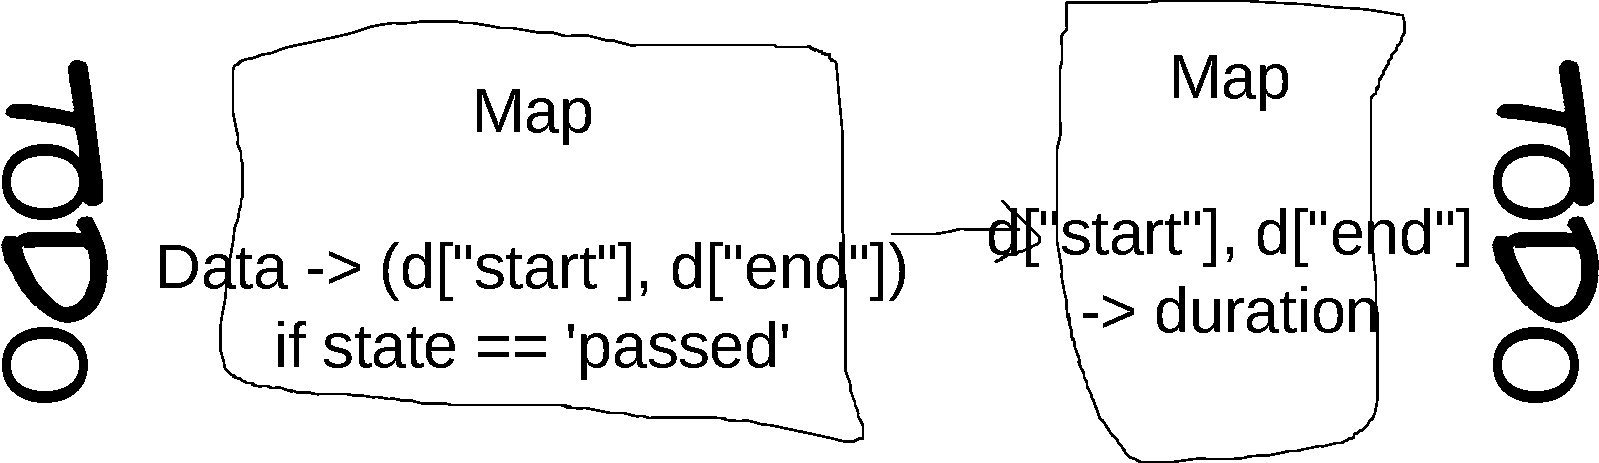
\includegraphics[width=0.8\textwidth]{assets/images/eval-rq3-mapreduce.pdf}
	\caption{MapReduce pipeline to find the average duration of a successful test run}
	\label{fig:eval-mapreduce-3}
\end{figure}

\noindent In addition to the first source, another $\SI{3702595}{}$ jobs have been analysed from the \emph{TravisTorrent} project. This project \cite{msr17challenge} scrapes the API of \travisci{} and combines this with data obtained from the \github{} API to augment the dataset with extra information. One of these additional values is the identifier of the previous executed build of every project. This identifier is required to answer the second research question. Furthermore, the amount of failed test cases in every run is included, which can be used to distinguish whether the test run has actually failed or the project could not be compiled and thus allowing a more fine-grained answer to the first research question as well. After analysis of this dataset, the execution time was not accurate compared to the actual timings on the \travisci{} build page, so this dataset was not used in the third research question. For analysis, the creators of TravisTorrent have provided a Google BigQuery\footnote{\url{https://bigquery.cloud.google.com/}} interface to allow querying the dataset, which is required given its magnitude. The following queries have been executed to obtain the required data:

\lstinputlisting[caption=TravisTorrent query: Find the amount of failed runs, label=lst:travistorrent-sql1, language=sql]{assets/listings/travistorrent-failed-runs.sql}
\lstinputlisting[caption=TravisTorrent query: Find the probability of consecutive failures,label=lst:travistorrent-sql2, language=sql]{assets/listings/travistorrent-consecutive-failures.sql}

% !TeX root = ../../thesis.tex

\subsection{Dodona data}
As mentioned before, Dodona utilises the MiniTest testing framework in conjunction with SimpleCov to calculate the coverage. MiniTest will by default only emit the name of every failed test case, without any further information. Furthermore, SimpleCov is only capable of calculating the coverage for the entire test suite and does not allow to retrieve the coverage on a per-test basis. To answer the fourth research question and apply the \velocity{} predictors to Dodona, a Python script has been created to reconstruct every failed test run. This script first queries the API of \githubactions{} to find which test runs have failed. In this thesis, $\SI{62}{}$ failed runs have been used. For every failed commit, the script retrieves the parent commit and calculates the coverage on a per-test basis. This thesis will assume that the coverage of the parent commit resembles the coverage of the failed commit. The coverage is calculated by applying the following two transformations to the parent commits and subsequently rescheduling these in \githubactions{}:

\begin{itemize}
	\item \textbf{Cobertura formatter:} The current SimpleCov reports can only be generated as HTML reports, preventing convenient analysis. This problem is resolved by using the Cobertura formatter instead, which generates XML reports. The structure of these reports is already supported by the Controller.
	
	\item \textbf{Parallel execution:} To reduce the execution time, the test cases are concurrently executed by four processes. The code coverage is recorded per process and afterwards merged. However, SimpleCov is not entirely thread-safe. This is not a problem if the total coverage is required, but it does prevent the accurate generation of per-test coverage. As a result, parallel execution has been disabled.
	
\end{itemize}
\clearpage
% !TeX root = ../thesis.tex

\section{Results}

\subsection{RQ1: Probability of failure}\label{ssec:results-rq1}
\autoref{fig:rq1-failure-probability} contains two pie charts that illustrate the amount of failed and successful test runs. The left chart contains the results of the dataset provided by Durieux et al \cite{travisanalysis}. This dataset contains $\SI{4558279}{}$ failed test runs versus $\SI{24323724}{}$ successful runs, which corresponds to a failure probability of $\SI{18.74}{\percent}$. The other pie chart visualises data from the TravisTorrent project. According to this dataset, the run has failed prior to starting the test suite in $\SI{42.89}{\percent}$ of the executions. For the remaining part of the runs, $\SI{225766}{}$ out of $\SI{2114920}{}$ executions contained at least one failed test case, corresponding to a failure percentage of $\SI{10.67}{\percent}$.

\begin{figure}[htbp!]
	\centering
	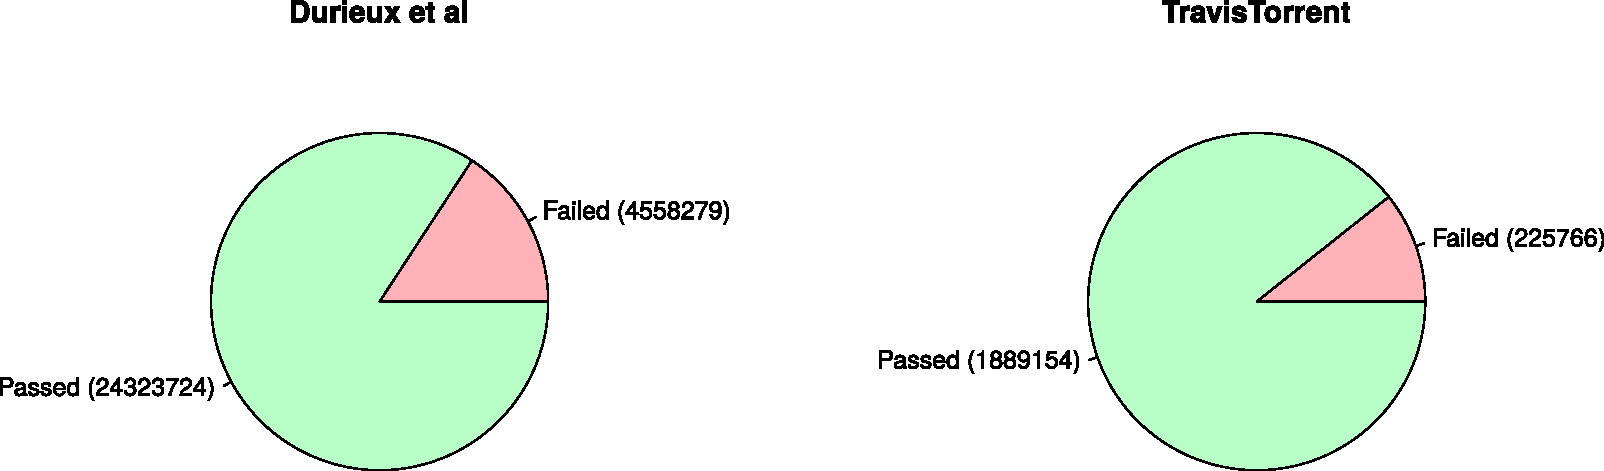
\includegraphics[width=\textwidth]{assets/charts/rq1-failure-probability.pdf}
	\caption{Probability of test run failure}
	\label{fig:rq1-failure-probability}
\end{figure}

\subsection{RQ2: Probability of consecutive failure}
In order to find consecutive failures, only the TravisTorrent project can be used as every entry in this dataset contains the identifier of the previous build which is required to link consecutive builds. The dataset contains $\SI{211040}{}$ test runs of which the test suite of the preceding test run was both executed and contained at least one failed test case. As illustrated in \autoref{fig:rq2-consecutive-failure}, $\SI{109224}{}$ of these test runs failed as well, versus $\SI{101816}{}$ test runs ($\SI{51.76}{\percent}$) that did succeed.

\begin{figure}[htbp!]
	\centering
	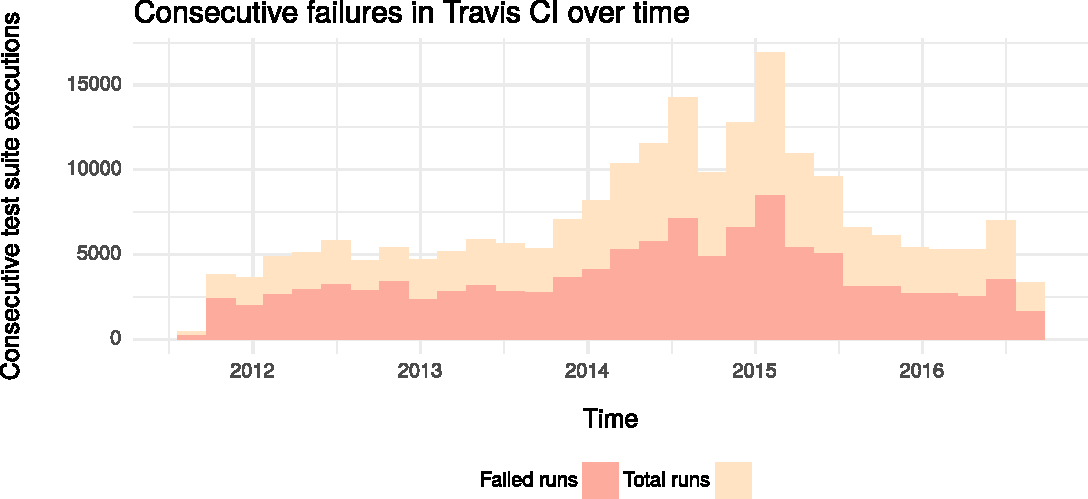
\includegraphics[width=\textwidth]{assets/charts/rq2-consecutive-failure.pdf}
	\caption{Consecutive test run failures on \travisci{}}
	\label{fig:rq2-consecutive-failure}
\end{figure}

\subsection{RQ3: Average test run duration}
The \travisci{} dataset provided by Durieux et al \cite{travisanalysis} has been filtered to exclude test runs with an execution time of less than $\SI{10}{\second}$, as this generally implies that the test suite did not actually execute due to an initialisation failure. \autoref{tbl:rq3-characteristics} contains the characteristics of the remaining analysed test runs. This table suggests that \travisci{} is primarily used for small projects, yet the maximal value is a strong outlier. \autoref{fig:rq3-durations} confirms the existence of $\SI{71378}{}$ test runs with an execution time of more than one hour. Further investigation has pointed out that these are mostly projects which are using mutation testing (\autoref{sssec:mutation-testing}), such as \texttt{plexus/yaks}\footnote{A Ruby library for hypermedia (\url{https://github.com/plexus/yaks}).}.

\begin{table}[h]
	\centering
	\begin{tabularx}{\textwidth}{|C|C|C|C|C|}
		\hline
		\textbf{\# runs} & \textbf{Minimum} & \textbf{Mean} & \textbf{Median} & \textbf{Maximum}\\
		\hline
		$\SI{24320504}{}$ & $\SI{10}{\second}$ & $\SI{385}{\second}$ & $\SI{178}{\second}$ & $\SI{26}{\hour} \SI{11}{\minute} \SI{26}{\second}$\\
		\hline
	\end{tabularx}
	\caption{Characteristics of the test run durations in \cite{travisanalysis}.}
	\label{tbl:rq3-characteristics}
\end{table}

\begin{figure}[htbp!]
	\centering
	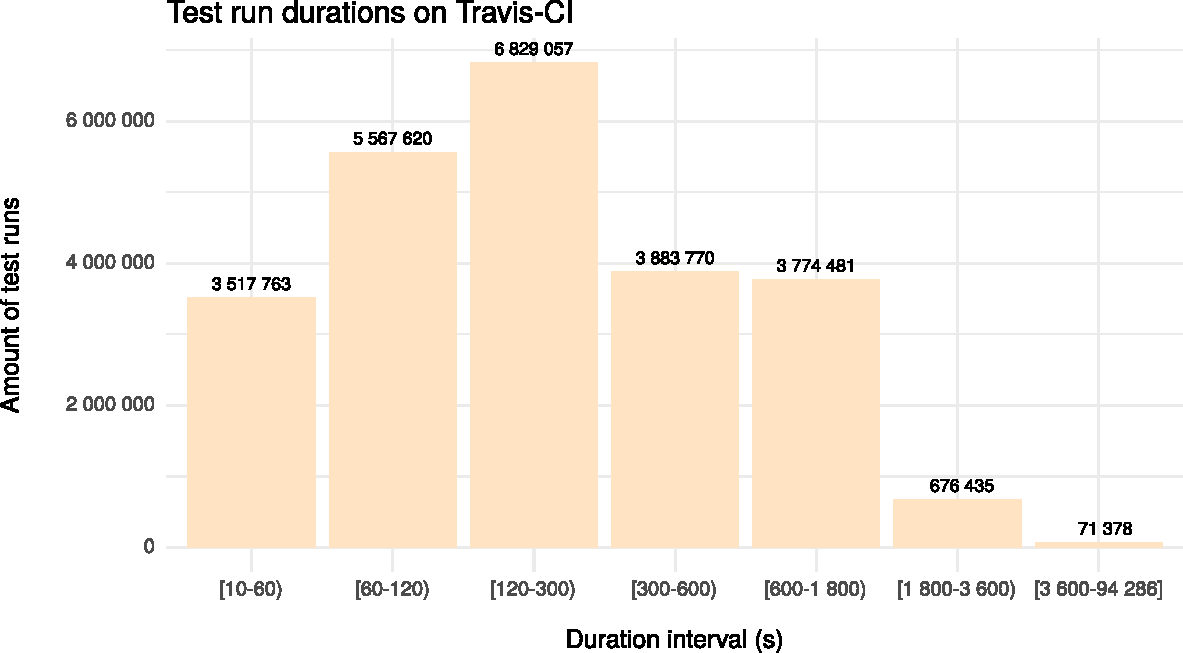
\includegraphics[width=\textwidth]{assets/charts/rq3-test-run-durations.pdf}
	\caption{Test run durations on \travisci{}}
	\label{fig:rq3-durations}
\end{figure}


\subsection{RQ4: Applying \tcp{} to Dodona}
Given the $\SI{62}{}$ collected test runs, another $\SI{9}{}$ runs have been omitted because these have been identified as a bug in the configuration of the test suite, preventing any test to be executed at all. This is something which cannot be detected by a prioritisation framework, since this requires more contextual information about the project.\\

\noindent \autoref{fig:rq4-performance} compares the performance of respectively the Alpha algorithm, the Greedy algorithm, the HGS algorithm and the ROCKET algorithm to the original, non-prioritised execution. The Alpha and HGS algorithm provide the most accurate predictions, with the latter algorithm being the least consistent. The Greedy algorithm on the other hand succeeds in predicting some executions very accurately, while failing to predict other runs anywhere near, which is the expected behaviour of a greedy heuristic. Finally, the ROCKET algorithm is not suitable for this project.\\

\begin{figure}[htbp!]
\centering
\subfloat[Alpha algorithm]{%
	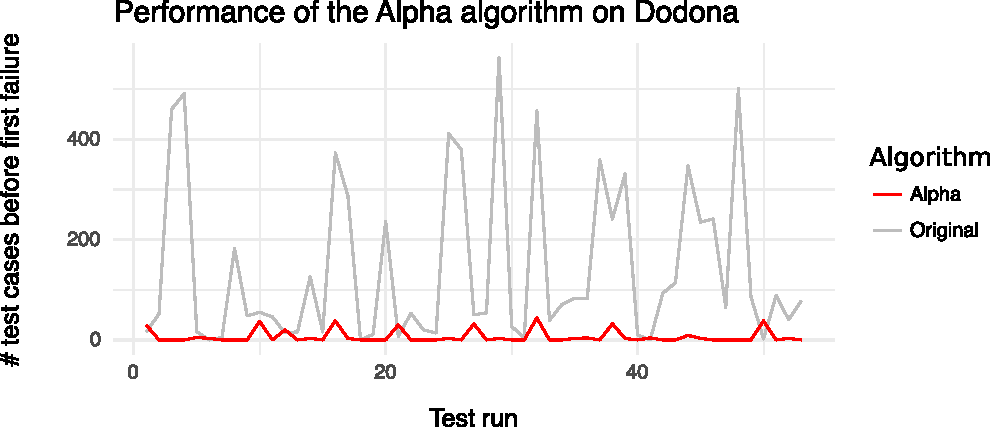
\includegraphics[width=\textwidth]{assets/charts/rq4-dodona-alpha.pdf}
}
\end{figure}
\begin{figure}
\ContinuedFloat
\subfloat[Greedy algorithm]{%
	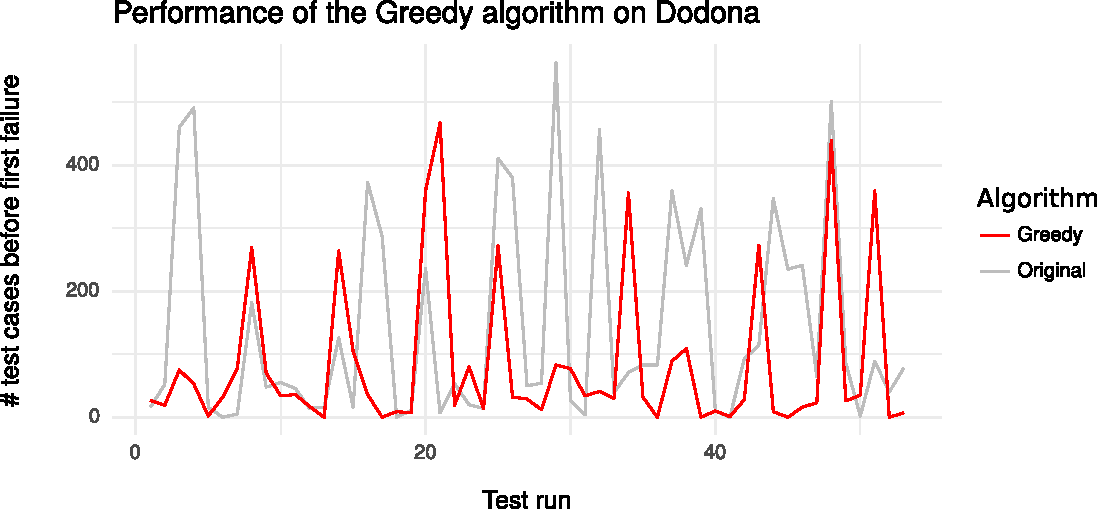
\includegraphics[width=\textwidth]{assets/charts/rq4-dodona-greedy.pdf}
}
\end{figure}
\begin{figure}
\ContinuedFloat
\subfloat[HGS algorithm]{%
	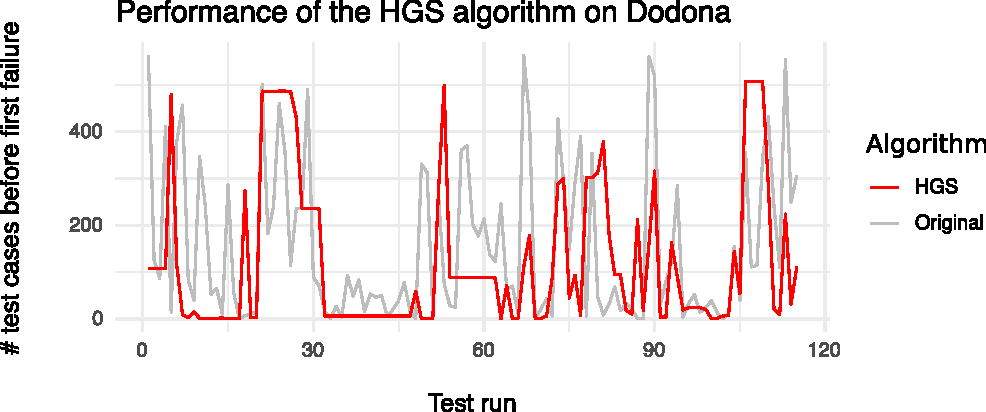
\includegraphics[width=\textwidth]{assets/charts/rq4-dodona-hgs.pdf}
}
\end{figure}
\begin{figure}
\ContinuedFloat
\centering
\subfloat[ROCKET algorithm]{%
	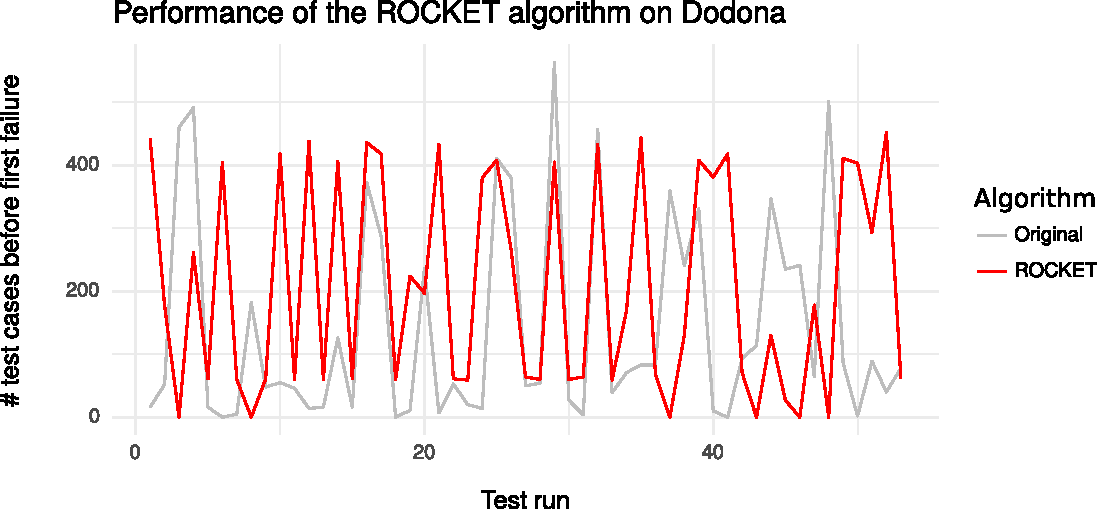
\includegraphics[width=\textwidth]{assets/charts/rq4-dodona-rocket.pdf}
}
\caption{Prediction performance on the Dodona project}
\label{fig:rq4-performance}
\end{figure}

\noindent \autoref{tbl:rq4-first-failure} contains the minimum, mean, median and maximum median amount of test cases until the first failure is observed. This table indicates that, except for the GreedyCoverAffected algorithm\footnote{The AllInOrder algorithm can be considered a deterministic random algorithm and therefore not an actual predictor.}, every predictor is able to perform at least one successful prediction. Furthermore, the maximum amount of executed test cases is lower than the original, for every predictor. The previous paragraph has already observed that the Alpha and HGS algorithm provide the best prediction accuracy for Dodona, this hypothesis is confirmed by the low median and mean values for these algorithms. These values confirm as well that the ROCKET algorithm is not able of providing accurate predictions.

\begin{table}[h]
	\centering
	\begin{tabularx}{\textwidth}{|X||c|c|c|c|}
		\hline
		\textbf{Algorithm} & \textbf{Minimum} & \textbf{Mean} & \textbf{Median} & \textbf{Maximum}\\
		
		\hline
		
		\emph{Original} & $\SI{0}{}$ & $\SI{143}{}$ & $\SI{65}{}$ & $\SI{563}{}$\\
		
		\hline
		
		Alpha & $\SI{0}{}$ & $\SI{7}{}$ & $\SI{6}{}$ & $\SI{44}{}$\\
		
		\hline
		AffectedRandom & $\SI{0}{}$ & $\SI{82}{}$ & $\SI{18}{}$ & $\SI{428}{}$\\
		AllInOrder & $\SI{1}{}$ & $\SI{102}{}$ & $\SI{71}{}$ & $\SI{455}{}$\\
		AllRandom & $\SI{0}{}$ & $\SI{71}{}$ & $\SI{16}{}$ & $\SI{477}{}$\\
		
		\hline
		
		GreedyCoverAffected & $\SI{31}{}$ & $\SI{307}{}$ & $\SI{296}{}$ & $\SI{446}{}$\\
		GreedyCoverAll & $\SI{0}{}$ & $\SI{85}{}$ & $\SI{32}{}$ & $\SI{467}{}$\\
		GreedyTimeAll & $\SI{0}{}$ & $\SI{209}{}$ & $\SI{172}{}$ & $\SI{452}{}$\\
		
		\hline
		
		HGSAffected & $\SI{0}{}$ & $\SI{54}{}$ & $\SI{10}{}$ & $\SI{511}{}$\\
		HGSAll & $\SI{0}{}$ & $\SI{109}{}$ & $\SI{6}{}$ & $\SI{487}{}$\\
		
		\hline
		
		ROCKET & $\SI{0}{}$ & $\SI{208}{}$ & $\SI{170}{}$ & $\SI{452}{}$\\
		
		\hline
	\end{tabularx}
	\caption{Amount of executed test cases until the first failure.}
	\label{tbl:rq4-first-failure}
\end{table}

\noindent Similarly, \autoref{tbl:rq4-first-failure-duration} contains the minimum, mean, maximum and median duration until the first failed test case is observed. This data further confirms the observations made in the previous paragraph and the effectiveness of the GreedyTimeAll predictor. Notice that the ROCKET algorithm performs better time-wise than quantity wise.

\begin{table}[h]
	\centering
	\begin{tabularx}{\textwidth}{|X||c|c|c|c|}
		\hline
		\textbf{Algorithm} & \textbf{Minimum} & \textbf{Mean} & \textbf{Median} & \textbf{Maximum}\\
		
		\hline
		
		\emph{Original} & $\SI{0}{\second}$ & $\SI{154}{\second}$ & $\SI{125}{\second}$ & $\SI{622}{\second}$\\
		
		\hline
		
		Alpha & $\SI{0}{\second}$ & $\SI{5}{\second}$ & $\SI{0}{\second}$ & $\SI{84}{\second}$\\
		
		\hline
		AffectedRandom & $\SI{0}{\second}$ & $\SI{64}{\second}$ & $\SI{10}{\second}$ & $\SI{355}{\second}$\\
		AllInOrder & $\SI{0}{\second}$ & $\SI{177}{\second}$ & $\SI{171}{\second}$ & $\SI{456}{\second}$\\
		AllRandom & $\SI{0}{\second}$ & $\SI{64}{\second}$ & $\SI{11}{\second}$ & $\SI{611}{\second}$\\
		
		\hline
		
		GreedyCoverAffected & $\SI{6}{\second}$ & $\SI{123}{\second}$ & $\SI{109}{\second}$ & $\SI{264}{\second}$\\
		GreedyCoverAll & $\SI{0}{\second}$ & $\SI{60}{\second}$ & $\SI{25}{\second}$ & $\SI{306}{\second}$\\
		GreedyTimeAll & $\SI{0}{\second}$ & $\SI{44}{\second}$ & $\SI{15}{\second}$ & $\SI{178}{\second}$\\
		
		\hline
		
		HGSAffected & $\SI{0}{\second}$ & $\SI{58}{\second}$ & $\SI{6}{\second}$ & $\SI{581}{\second}$\\
		HGSAll & $\SI{0}{\second}$ & $\SI{130}{\second}$ & $\SI{16}{\second}$ & $\SI{578}{\second}$\\
		
		\hline
		
		ROCKET & $\SI{0}{\second}$ & $\SI{47}{\second}$ & $\SI{16}{\second}$ & $\SI{178}{\second}$\\
		
		\hline
	\end{tabularx}
	\caption{Duration until the first failure.}
	\label{tbl:rq4-first-failure-duration}
\end{table}

    duration         Original        AllRandom     
Min.   :118165   Min.   :  0.00   Min.   : 0.000  
1st Qu.:195877   1st Qu.:  0.00   1st Qu.: 0.000  
Median :297371   Median :  2.00   Median : 4.000  
Mean   :303527   Mean   : 67.57   Mean   : 9.257  
3rd Qu.:414956   3rd Qu.:110.00   3rd Qu.:13.500  
Max.   :505996   Max.   :278.00   Max.   :64.000  

AllInOrder     GreedyCoverAll   AffectedRandom  
Min.   : 0.000   Min.   : 0.000   Min.   : 0.000  
1st Qu.: 0.000   1st Qu.: 0.000   1st Qu.: 0.000  
Median : 1.000   Median : 1.000   Median : 2.000  
Mean   : 9.229   Mean   : 8.971   Mean   : 8.886  
3rd Qu.:12.000   3rd Qu.:13.000   3rd Qu.:11.500  
Max.   :37.000   Max.   :44.000   Max.   :45.000  

HGSAffected     GreedyCoverAffected     HGSAll    
Min.   : 0.000   Min.   : 0.00       Min.   : 0.0  
1st Qu.: 0.000   1st Qu.: 0.00       1st Qu.: 0.0  
Median : 3.000   Median : 2.00       Median : 7.0  
Mean   : 8.886   Mean   :15.09       Mean   : 9.6  
3rd Qu.:11.500   3rd Qu.:31.00       3rd Qu.:12.5  
Max.   :64.000   Max.   :43.00       Max.   :43.0  

Alpha            Rocket       GreedyTimeAll   
Min.   : 0.000   Min.   :  0.00   Min.   :  0.00  
1st Qu.: 0.000   1st Qu.:  3.50   1st Qu.:  3.50  
Median : 1.000   Median : 27.00   Median : 27.00  
Mean   : 8.971   Mean   : 42.23   Mean   : 42.23  
3rd Qu.:13.000   3rd Qu.: 49.00   3rd Qu.: 49.00  
Max.   :44.000   Max.   :216.00   Max.   :216.00  

Original\_ms      AllRandom\_ms    AllInOrder\_ms   
Min.   :     0   Min.   :     0   Min.   :     0  
1st Qu.:     0   1st Qu.:     0   1st Qu.:     0  
Median :  9560   Median :   739   Median :   862  
Mean   : 73612   Mean   : 13299   Mean   : 32391  
3rd Qu.:122586   3rd Qu.: 13592   3rd Qu.: 78063  
Max.   :283433   Max.   :184805   Max.   :139345  

GreedyCoverAll\_ms AffectedRandom\_ms HGSAffected\_ms  
Min.   :     0    Min.   :     0    Min.   :     0  
1st Qu.:     0    1st Qu.:     0    1st Qu.:     0  
Median :   620    Median :   317    Median :  1318  
Mean   : 15251    Mean   : 19732    Mean   : 23738  
3rd Qu.:  8620    3rd Qu.:  6460    3rd Qu.: 11786  
Max.   :197463    Max.   :174491    Max.   :211702  

GreedyCoverAffected\_ms   HGSAll\_ms         Alpha\_ms     
Min.   :    0          Min.   :     0   Min.   :     0  
1st Qu.:    0          1st Qu.:     0   1st Qu.:     0  
Median : 4229          Median :  2818   Median :   647  
Mean   :21835          Mean   : 12494   Mean   : 15189  
3rd Qu.:37885          3rd Qu.:  8475   3rd Qu.:  8386  
Max.   :75637          Max.   :157003   Max.   :193618  

Rocket\_ms      GreedyTimeAll\_ms      idx      
Min.   :     0   Min.   :    0    Min.   : 1.0  
1st Qu.:     0   1st Qu.:    0    1st Qu.: 9.5  
Median :   254   Median :  257    Median :18.0  
Mean   :  6844   Mean   : 6852    Mean   :18.0  
3rd Qu.:  1760   3rd Qu.: 1754    3rd Qu.:26.5  
Max.   :100011   Max.   :99765    Max.   :35.0  

\clearpage
% !TeX root = thesis.tex

\chapter{Conclusion}

The main purpose of this thesis has been to investigate different approaches towards optimising the test suite of a common software project. The concepts of \tsm{}, \tcs{} and \tcp{} have been introduced and accompanying algorithms have been presented. A novel client-server oriented framework for the latter approach has been proposed, as well as a new prioritisation algorithm. Finally, \velocity{} has been applied to the UGent Dodona project, proving its ability to predict test case failure and therefore reduce the execution time of the test suite.\\

\noindent A second purpose of this thesis was to gain useful insights into the behaviour of a typical test suite. These insights have been formulated as three additional research questions, to which answers have been provided in the previous chapter.

\section{Future work}
The proposed \velocity{} implementation in this thesis is currently able to prioritise a Gradle Java project using 10 available predictors and a meta predictor. While this is certainly functional, it is far from complete and multiple improvements can be added.

\subsection{Java Agent}
The existing Java Agent can be extended in multiple ways. The most prominent addition would be to allow test cases to be executed in parallel. At the moment of writing, this is not possible yet. In order to facilitate parallel testing, one must first decide how to schedule the prioritised test cases across multiple threads, since the execution time of a test case varies strongly. One possibility to perform this scheduling is to use the average execution time per test case, which is obtained from prior runs. Alternatively, this can be performed at runtime by using any existing inter-thread communication paradigm such as message passing. On the implementation side of parallelisation, the current \texttt{TestProcessor} should be adapted to inherit from the \texttt{MaxNParallelTestClassProcessor}. A thread pool should ideally be used to reduce the overhead of restarting a new thread for every test case.

\subsection{Predictions}
Further research and improvements to the predictors can be made on four different aspects.\\

\noindent The first enhancement is that currently the predictor does not discriminate between a unit test or an integration test. 
Recall that the scope of a unit test is limited to a small fraction of the application and that its execution time is ideally rather low. An integration test however usually takes longer to execute and tests multiple components of the application at once. The predictor could make use of this distinction and assume that a failure in a unit test has a high probability of resulting in a failed integration test as well, hence prioritising unit tests over integration tests.\\

\noindent Secondly, the prediction algorithms currently take into account which source code lines have either been modified or removed in order to prioritise affected test cases. Likewise, test cases of which the code has been modified should also be considered as candidates for prioritisation, as the changed test case might contain a bug as well.\\

\noindent A third and unexplored research opportunity is to investigate the joint performance of multiple prediction algorithms combined. This could be integrated with the existing meta predictor. Instead of assigning a score to the entire prediction, multiple predictions could be intermingled using predefined weights.\\

\noindent The final improvement is to take into account branch coverage in addition to the statement coverage which is currently used. This is a rather complex feature as not every coverage framework is capable of reporting accurately which branches have been covered and which ones have not. A suggested implementation would be to instrument the source code and rewrite every condition of every branch as separate \texttt{if}-statements.

\subsection{Meta predictor}
The proposed meta predictor increases the score of every predictor which predicted an above-average ranking and decreases the score of the other predictors. However, a possible problem with this approach is that the nature of the source code might evolve and change as time progresses. Using the current updating strategy it will take several test suite invocations for an alternative predictor to be preferred by the meta predictor. If a saturating counter would be used instead (\autoref{fig:saturating-counter}), this would be resolved much more quickly, allowing a more versatile meta predictor.

\begin{figure}[htbp!]
	\centering
	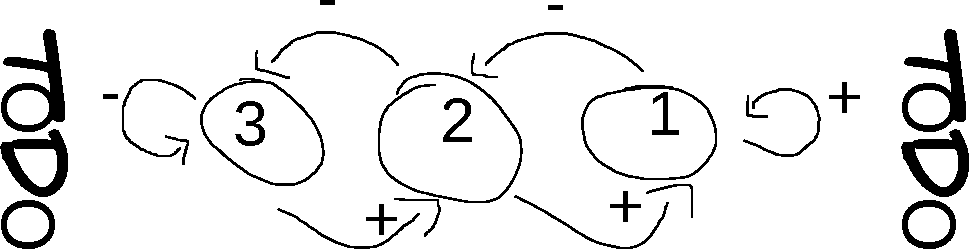
\includegraphics[width=\textwidth]{assets/images/saturating-counter.pdf}
	\caption{Saturating counter}
	\label{fig:saturating-counter}
\end{figure}

In addition to implementing a different update strategy, it might be worth to investigate the use of machine learning or linear programming models as a meta predictor, or even as a prediction algorithm.

\subsection{Final enhancements}
Finally, since some of the implemented algorithms are inherently \tsm{} algorithms rather than prioritisation algorithms, the framework might opt to not execute some test cases at all, whereas now the entire test suite is always executed.\\

\noindent Support for other programming languages and frameworks is possible by implementing new agents. The basic implementation is straightforward to restart the test suite after every executed test case, should test case reordering not be supported natively by the test framework.
\clearpage
% !TeX root = thesis.tex

\printbibliography[]
\clearpage
% !TeX = thesis.tex

\listoffigures
\clearpage
% !TeX root = thesis.tex

\listoftables
\clearpage
% !TeX root = thesis.tex

\addcontentsline{toc}{chapter}{\lstlistlistingname}
\lstlistoflistings
\clearpage
% !TeX root = thesis.tex

\begin{appendices}
\appendix
\crefalias{chapter}{appendix}

\chapter{TravisTorrent queries}
\label{appendix:travistorrent}
\lstinputlisting[caption=TravisTorrent query: Find the amount of failed runs, label=lst:travistorrent-sql1, language=sql]{assets/listings/travistorrent-failed-runs.sql}

\lstinputlisting[caption=TravisTorrent query: Find the probability of consecutive failures,label=lst:travistorrent-sql2, language=sql]{assets/listings/travistorrent-consecutive-failures.sql}

\end{appendices}

\end{document}
